\newline
\newline
\hfill

\section{Intro}
In this chapter, we discuss the application in terms of front-end, Design and scenarios that include the app.
As mentioned before, we use the Google Mobile UI (Flutter),
It is famous for its unique design everything needed for developing mobile apps. Flutter also has widgets for Material Design and Cupertino that allow developers to easily render the UI on both IOS and Android platform.
Before developing a new mobile app, you need to design it first. It’s critical to plan every step, and at some point, you might want to retreat and examine what you’re building.

\section{Mobile App}
\subsection{ App Design }
There are two phases of any mobile app design.
\begin{enumerate}
\item Mobile app design strategy
\item App design process
\end{enumerate}
\textbf{\textit{Mobile App Design Strategy}}
It starts with a strategy. It defines the future and the path to reach your destination.
Developing a mobile strategy links back to  \underline{the company strategy}  and has four stages:
\begin{enumerate}
\item Understand the business strategy
\item Business mobile app strategy
\item App strategy
\item Product management strategy
\end{enumerate}

\textbf{\textit{App design process}} \par
The basic app design process consists of following steps:

    
\begin{figure}
 \begin{subfigure}{\textwidth}
    \centering
        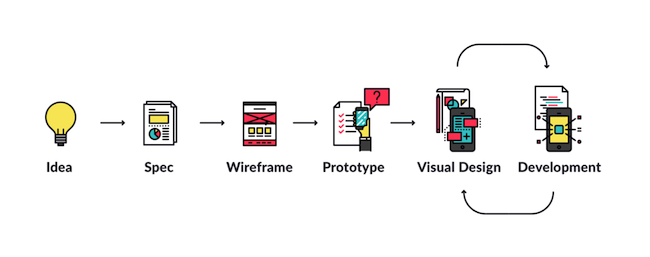
\includegraphics[width=1\linewidth]{images/ch3/design-process-preview-650px-opt.png} 
            \caption{The design process]{The design process }\label{fig: The design process}}

    \end{subfigure}
\par

\begin{subfigure}{0.5\textwidth}
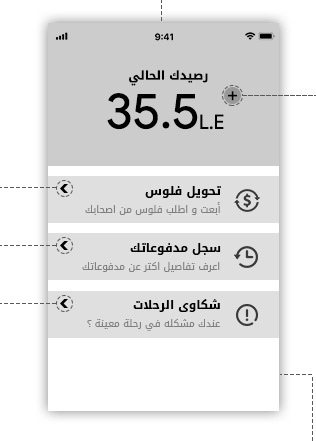
\includegraphics[width=1\linewidth, height=10cm]{images/ch3/wireframe.png} 
\caption{wireframe}
\label{fig:subim1}
\end{subfigure}
\begin{subfigure}{0.5\textwidth}
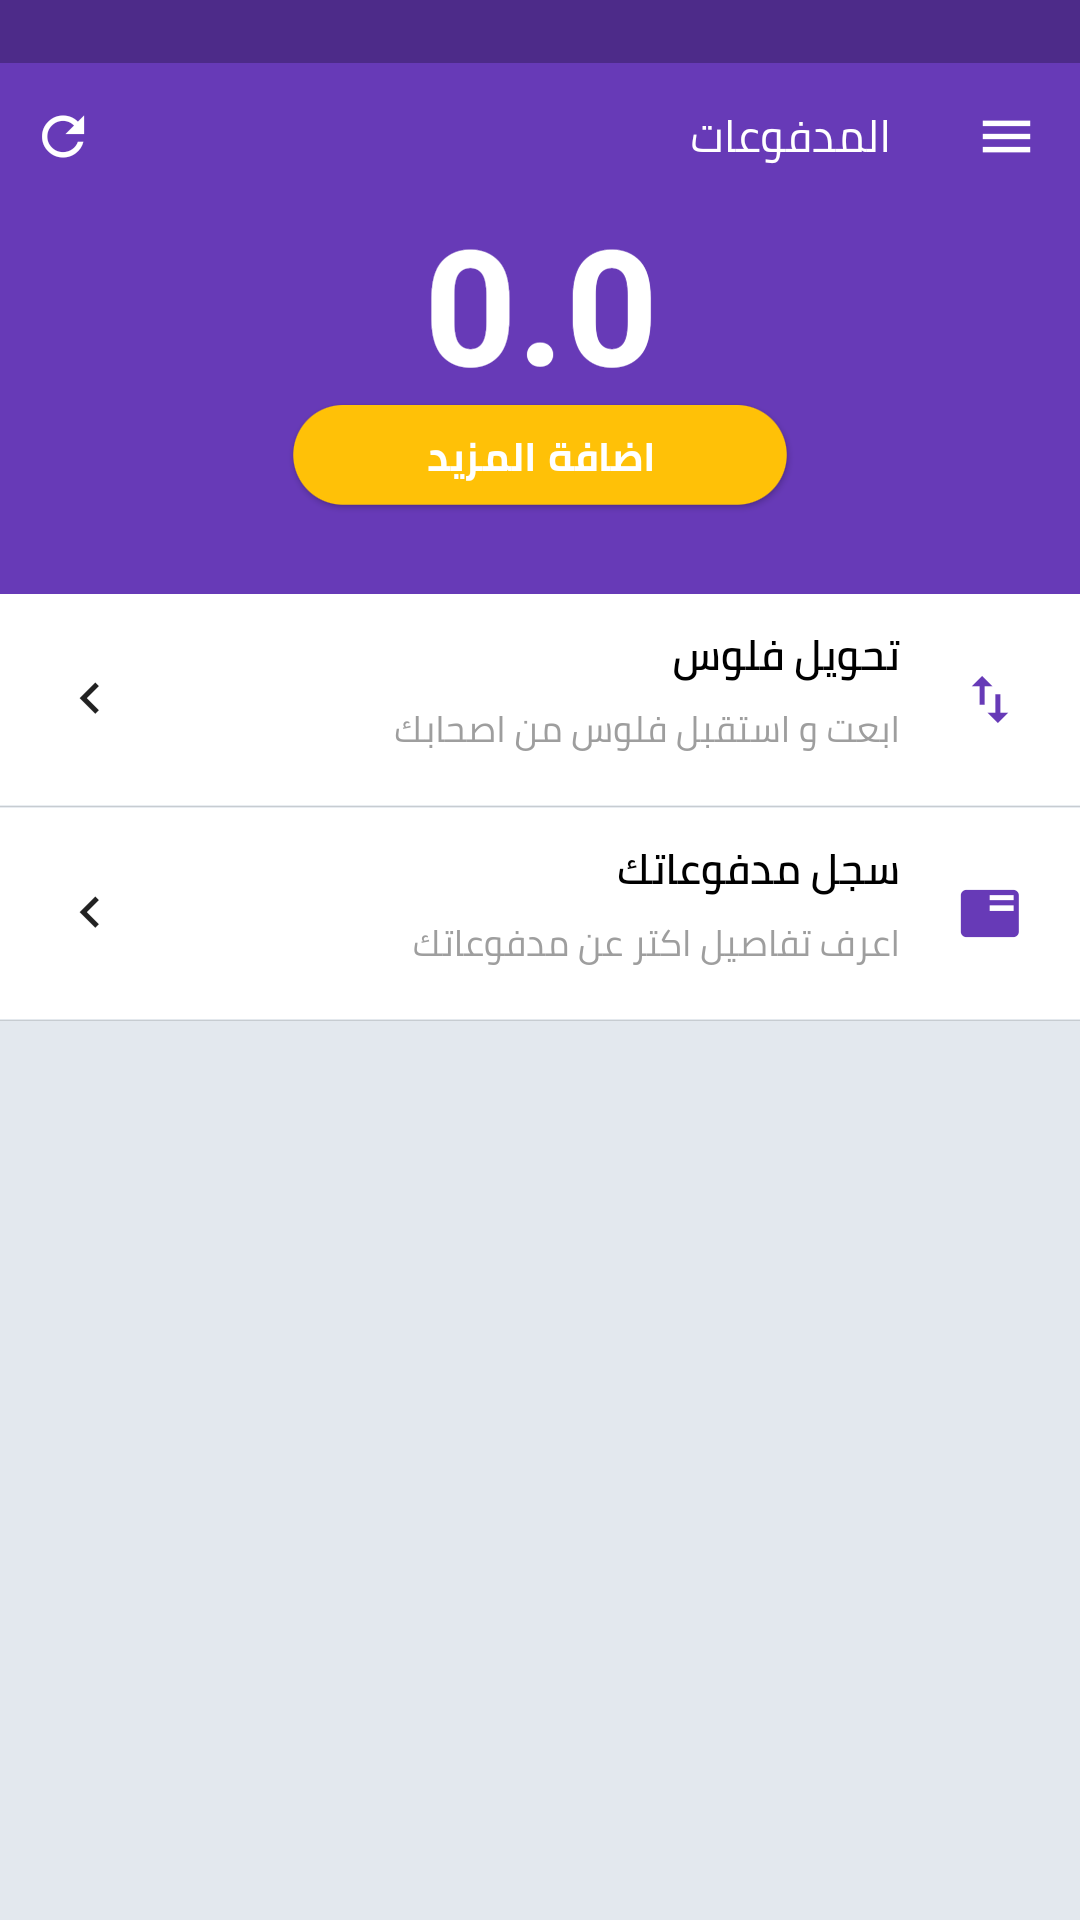
\includegraphics[width=.7\linewidth, height=10cm]{images/ch3/ui.png}
\caption{prototype}
\label{fig:subim2}
\end{subfigure}
\caption{wireframe and prototype}
\label{fig:image2}

    
   
\end{figure}


\begin{enumerate}
 \item idea
\item spec
\item  wireframe
\item Prototype
\item UI design
\item App development 
\end{enumerate}


  
\section{Mobile Front-end}
\newline

\subsection{Introduction}
\newline
Over the past ten years, the number of smartphones used has exceeded 2.5 billion. Every year, consumers spend  380 billion dollar on new devices. Each of them contains applications that simplify life, help calculate taxis or food, call them, and order them.
As for this application, it is intended for all age groups, it is easy to use and used for both Android and IOS, and anyone can download it.\par
The front end, also known as the client-side through which all our customers can use our apps and enjoy their services.
\par \newline
Not only are the beautiful screens, but the application connects to the server to be able to send and receive data to provide the desired service.
Fetching data from the internet is necessary for most apps. Luckily, Dart and Flutter provide tools, such as the HTTP package, for this type of work. 

\textbf{\textit{Mobile App Screens:}}\par

\textbf{\textit{login Page:}}  to enter the email and password also checks that the
user must be authorized.it also contain sing up page if the user does not have account(this page in each app).\par
if the user forgot the password, he can recovery by phone number or email.

 \begin{figure}[H] 
 \begin{subfigure}[b]{0.5\linewidth}
    \centering
    
\includegraphics[width=0.5\linewidth]{images/ch3/login/0.png}
  
  \end{subfigure}%% 
    \begin{subfigure}[b]{0.5\linewidth}
    \centering
    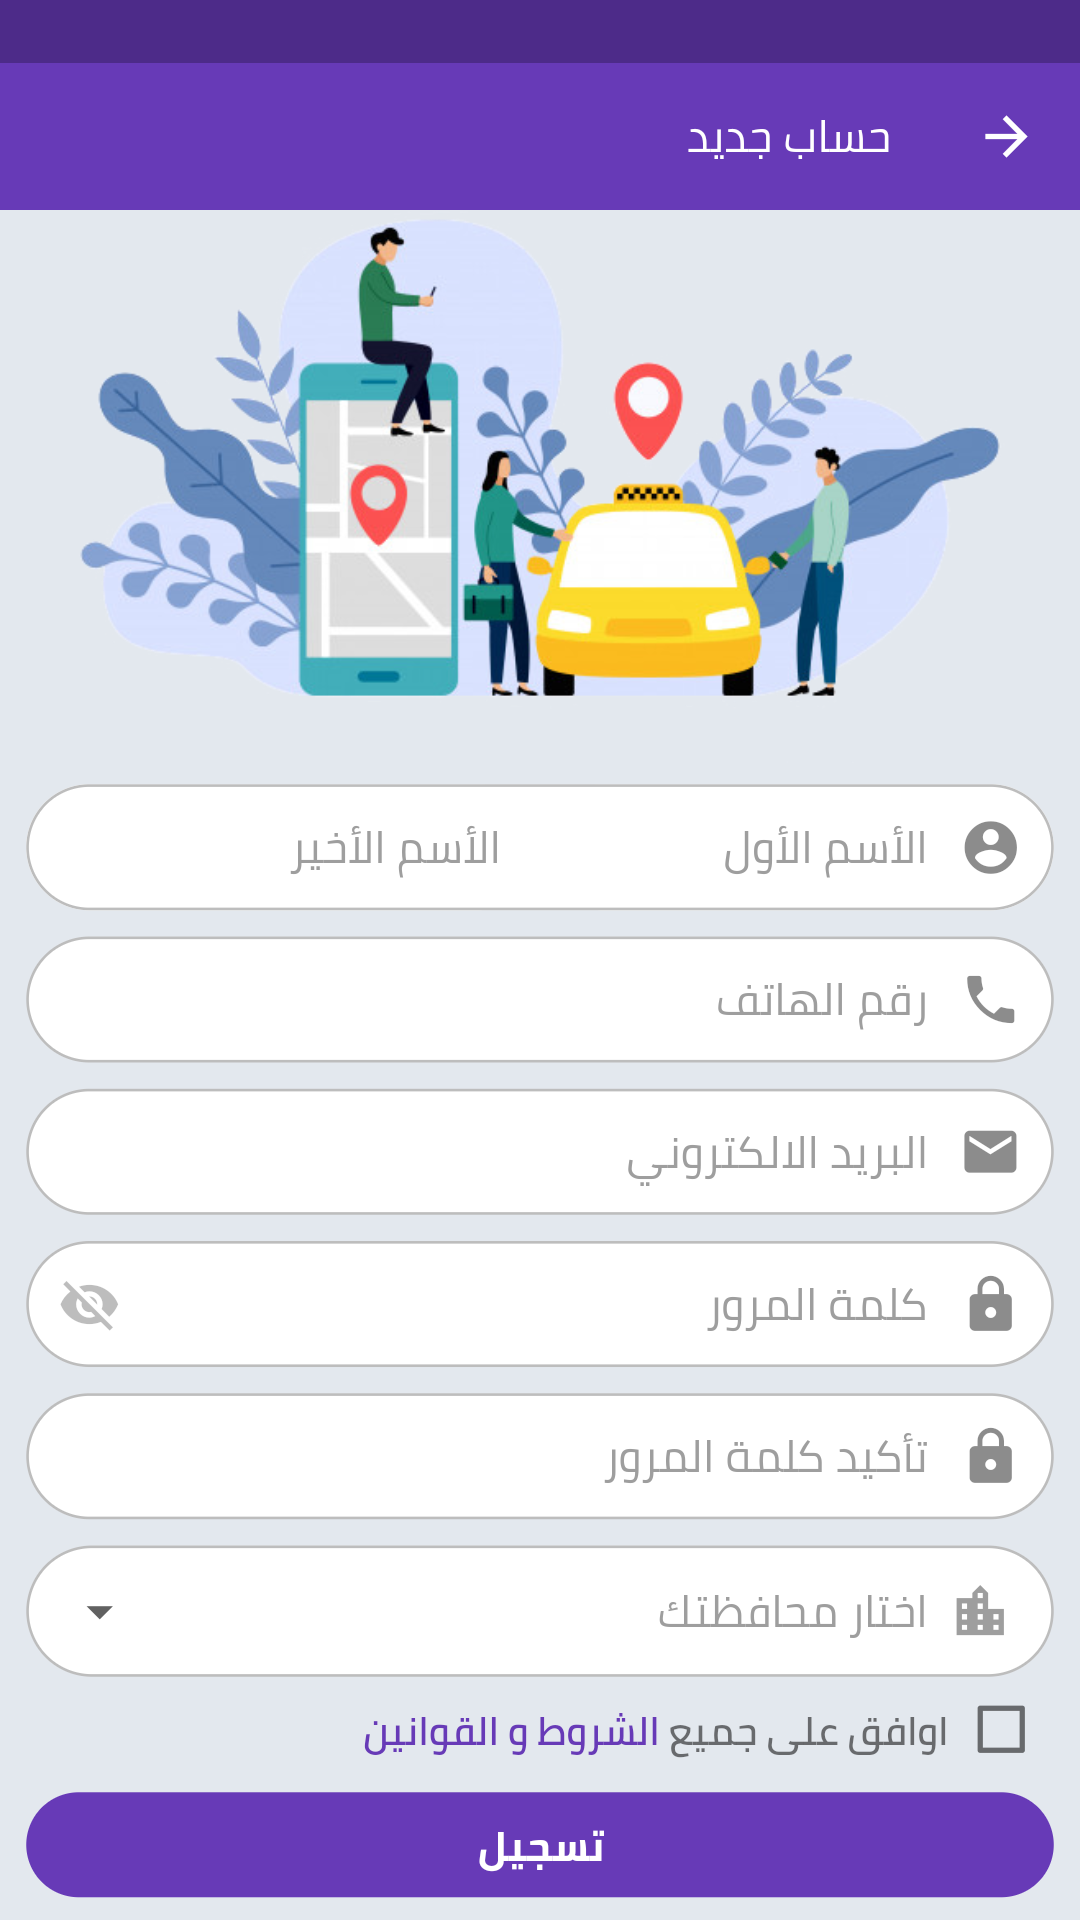
\includegraphics[width=0.5\linewidth]{images/ch3/login/1.png}
  
  \end{subfigure}%% 
      \begin{subfigure}[b]{0.5\linewidth}
    \centering
    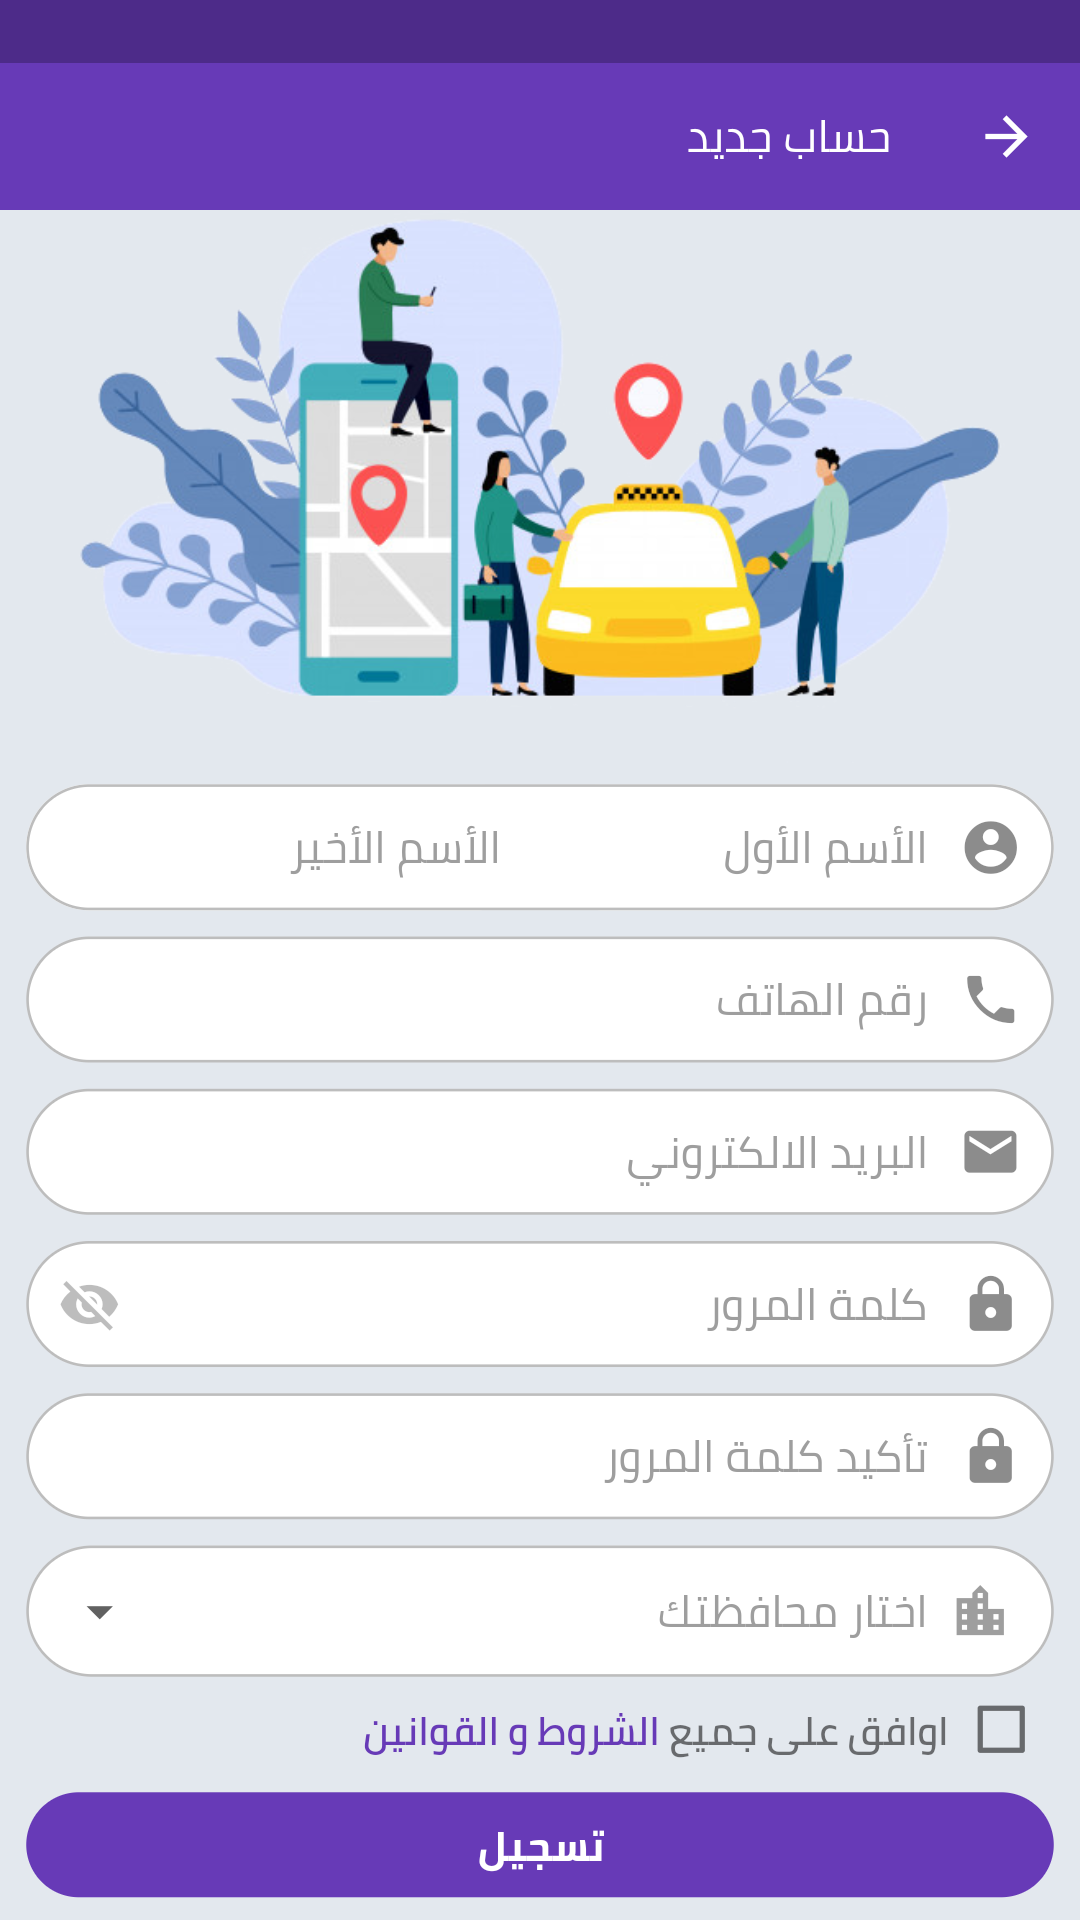
\includegraphics[width=0.4\linewidth]{images/ch3/login/1.png}
   \caption{ Login Page}
  \end{subfigure}%% 

    \caption{ Login and Registration Page}
\begin{figure}
    \centering
      
\includegraphics[width=0.5\linewidth]{images/ch3/login/2.png}
    \caption{ Reset password page }
    \label{fig:my_label}
\end{figure}
  \end{figure}


\textbf{\textit{home Page:}}the user's page  contains the available lines, the number of seats the user can use to book a new ride, select location, and payment way.
 On the other hand, the driver's homepage contains a choice of the number of seats available to him that are ready to receive user's new ride notifications can be received
\begin{figure}[H] 
  \begin{subfigure}[b]{0.5\linewidth}
    \centering
    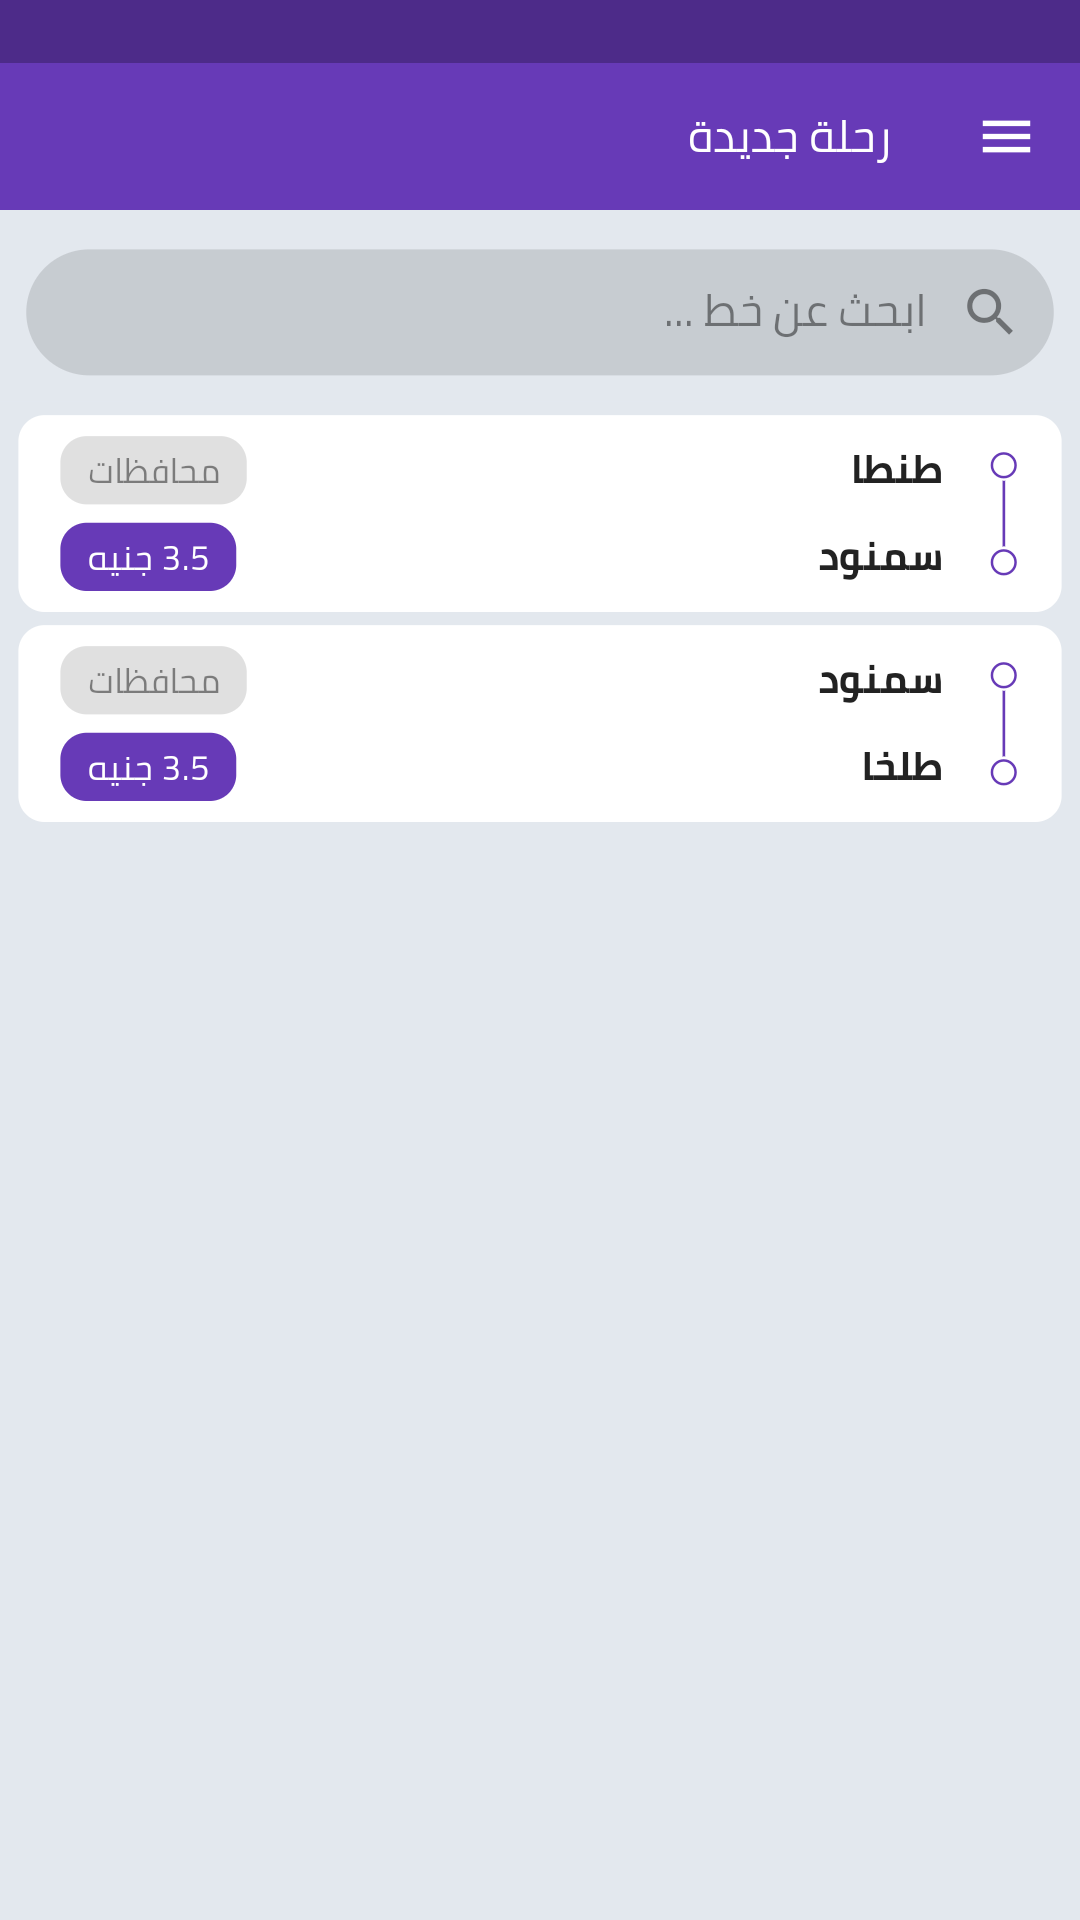
\includegraphics[width=0.75\linewidth]{images/ch3/0.png}
    \caption{Choose the available line} 
    \label{fig7:a} 
    \vspace{4ex}
  \end{subfigure}%% 
  \begin{subfigure}[b]{0.5\linewidth}
    \centering
    
\includegraphics[width=0.75\linewidth]{images/ch3/1.png}
    \caption{Confirm the location} 
    \label{fig7:b} 
    \vspace{4ex}
  \end{subfigure} 
  \caption{ User Home page}
  \label{fig7} 
\end{figure}

\par \textbf{\textit{Pairing Page:}}
\par  The processes to find the closest driver with requested seats until the driver accepts the user requests which showing until 10 seconds for each driver and the driver information appear to the user  who can accept this driver or not available driver now.
\begin{figure}[H] 
  \begin{subfigure}[b]{0.5\linewidth}
    \centering
    
\includegraphics[width=0.5\linewidth]{images/ch3/5.png}
    \caption{Searching for drivers} 
    \label{fig7:a} 
  \end{subfigure}%% 
  \begin{subfigure}[b]{0.5\linewidth}
    \centering
    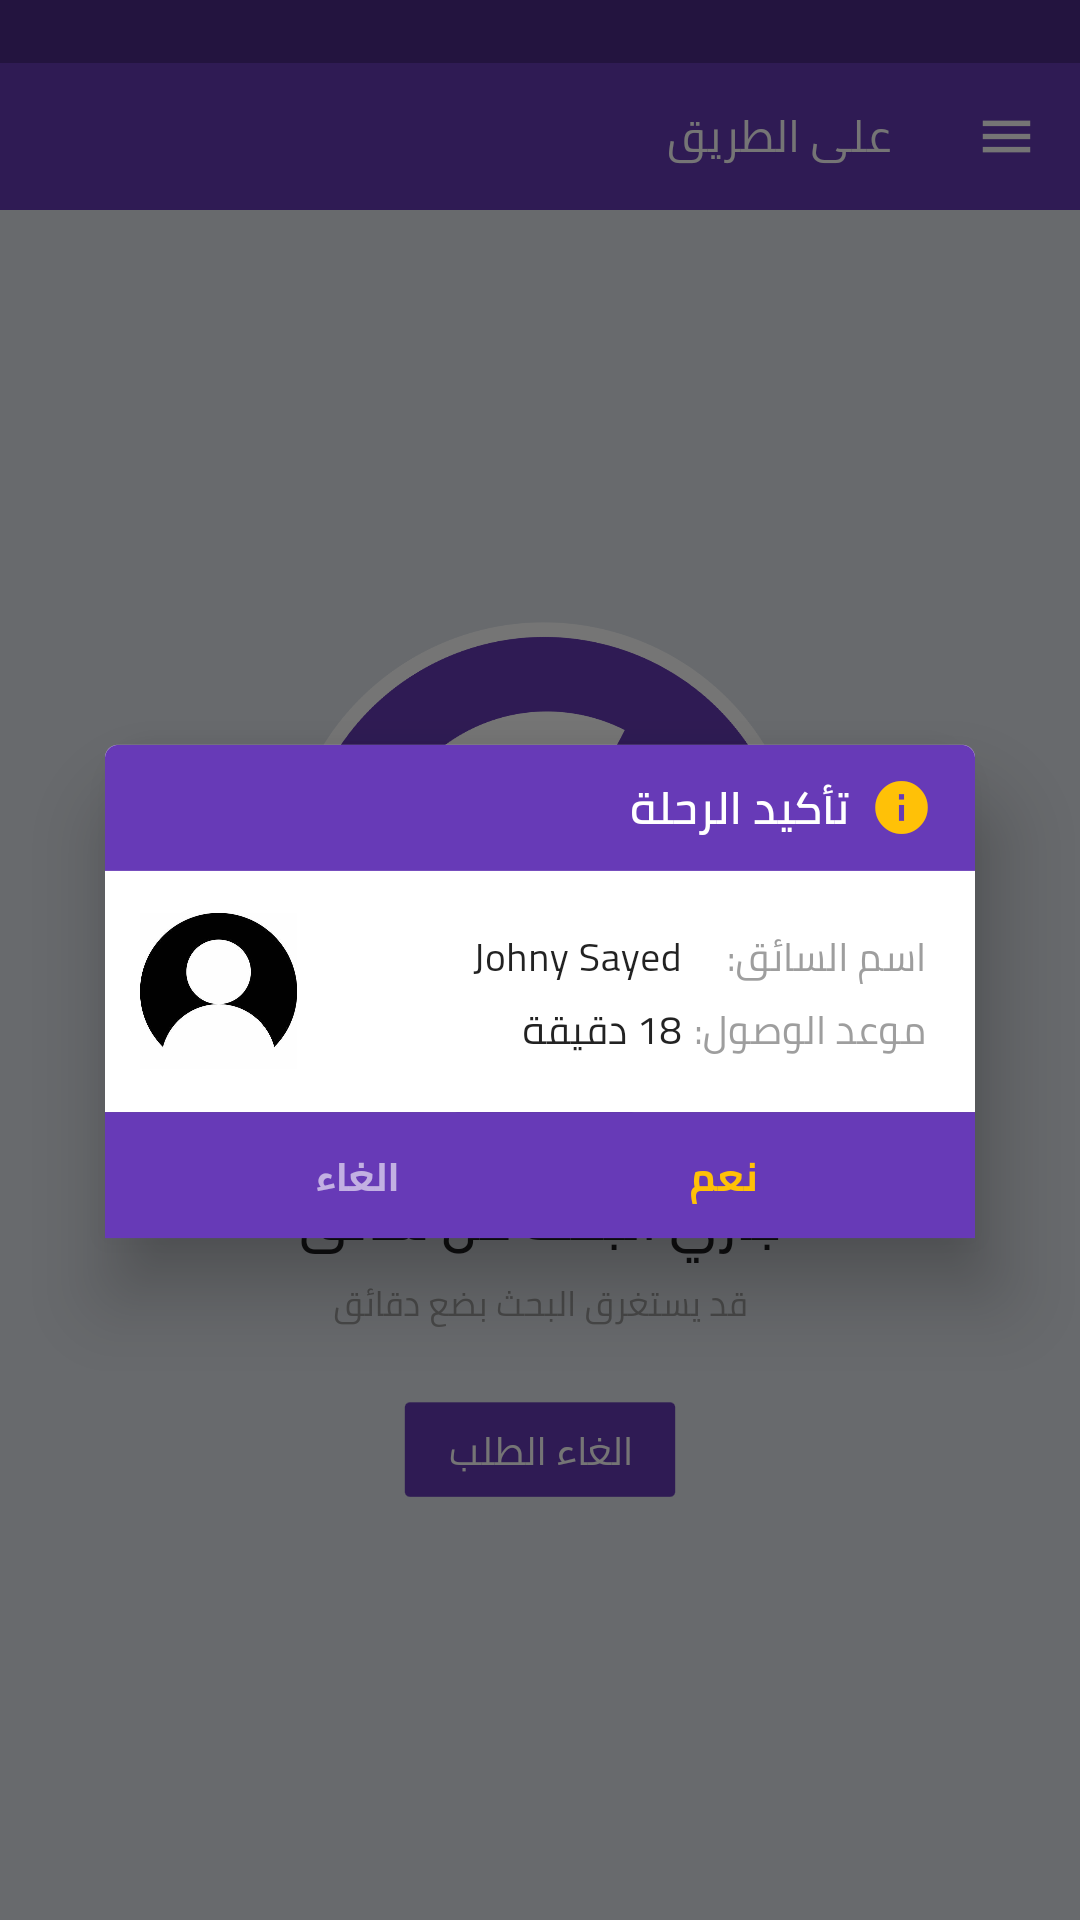
\includegraphics[width=0.5\linewidth]{images/ch3/6.png} 
    \caption{The user finds driver} 
    \label{fig7:d} 
  \end{subfigure} 
  \caption{ Pairing page}
  \label{fig7} 
\end{figure}

\textbf{\textit{tracking page :}}where the driver and the user are connected via google map until the driver arrived at the desired location.

\begin{figure}[H] 
  \begin{subfigure}[b]{0.5\linewidth}
    \centering
    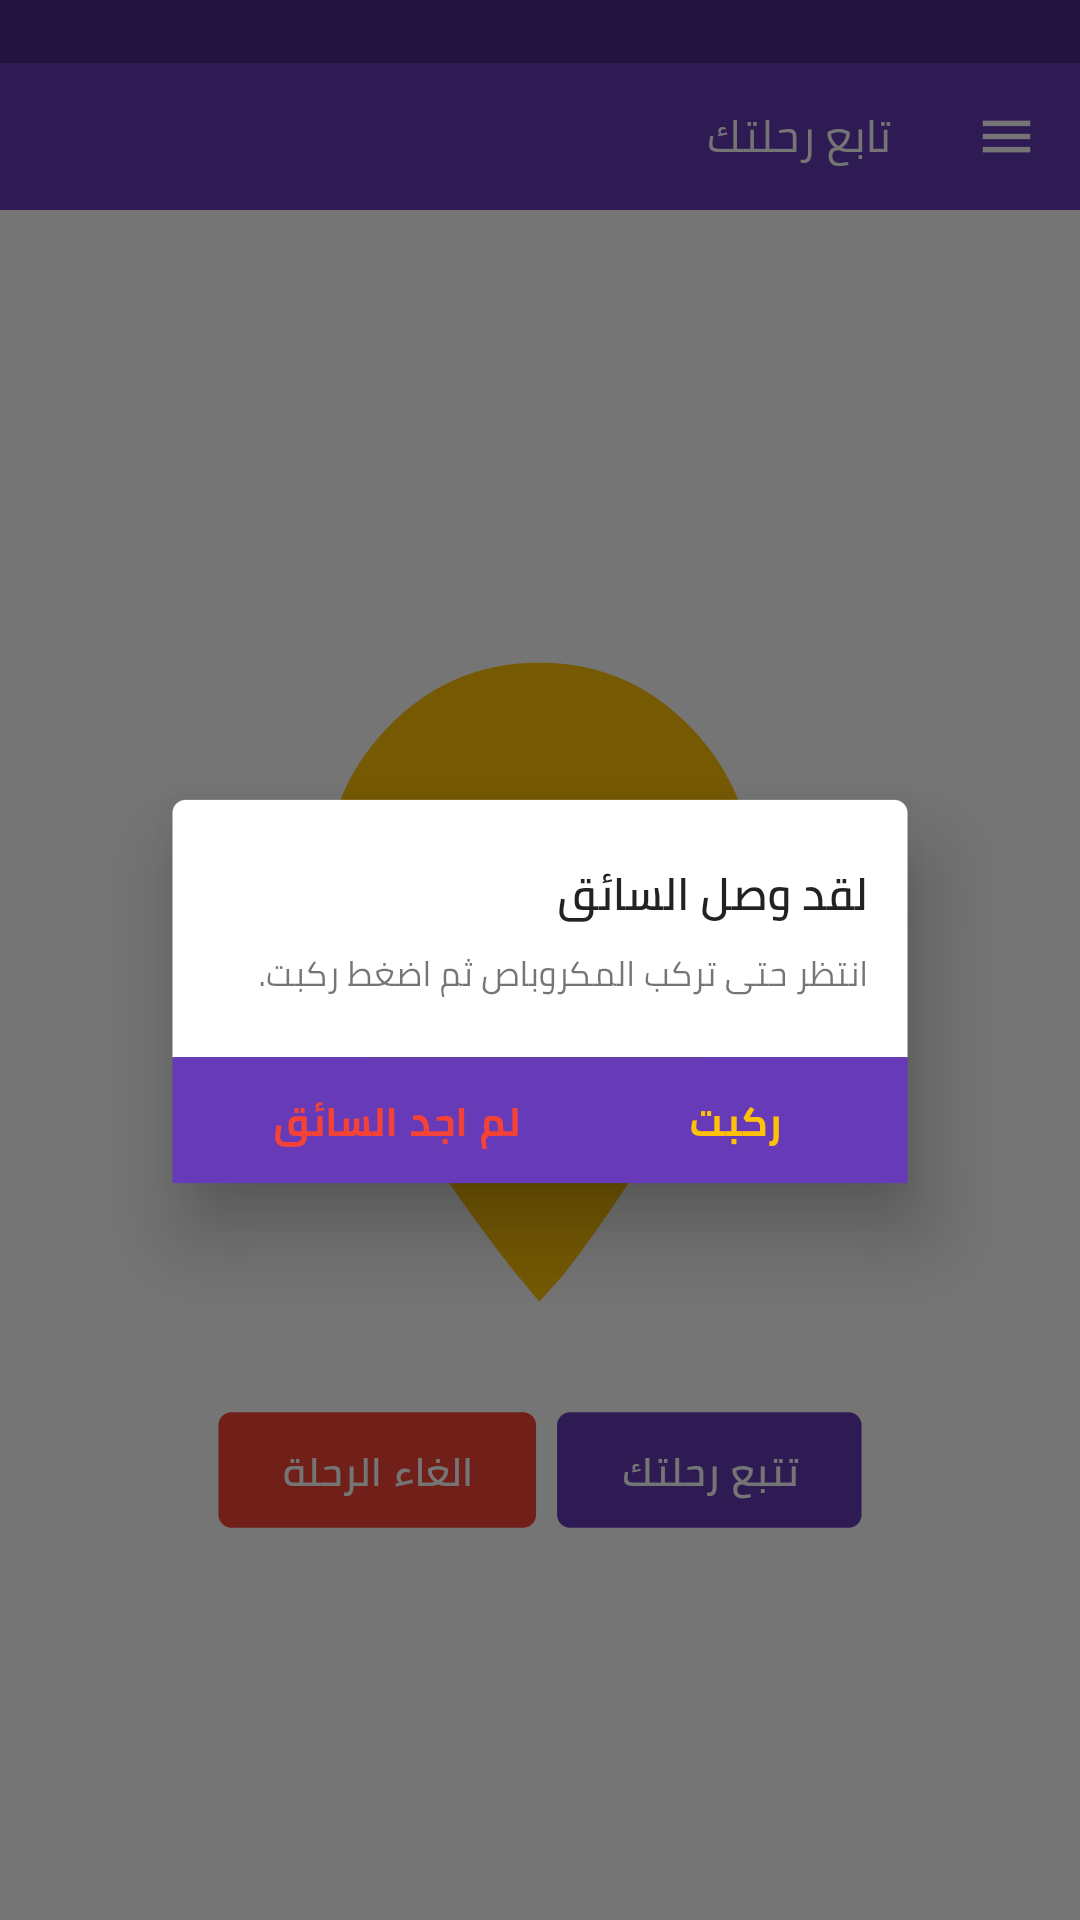
\includegraphics[width=0.5\linewidth]{images/ch3/7.png}
     
    \label{fig7:a} 
  \end{subfigure}%% 
  \begin{subfigure}[b]{0.5\linewidth}
    \centering
    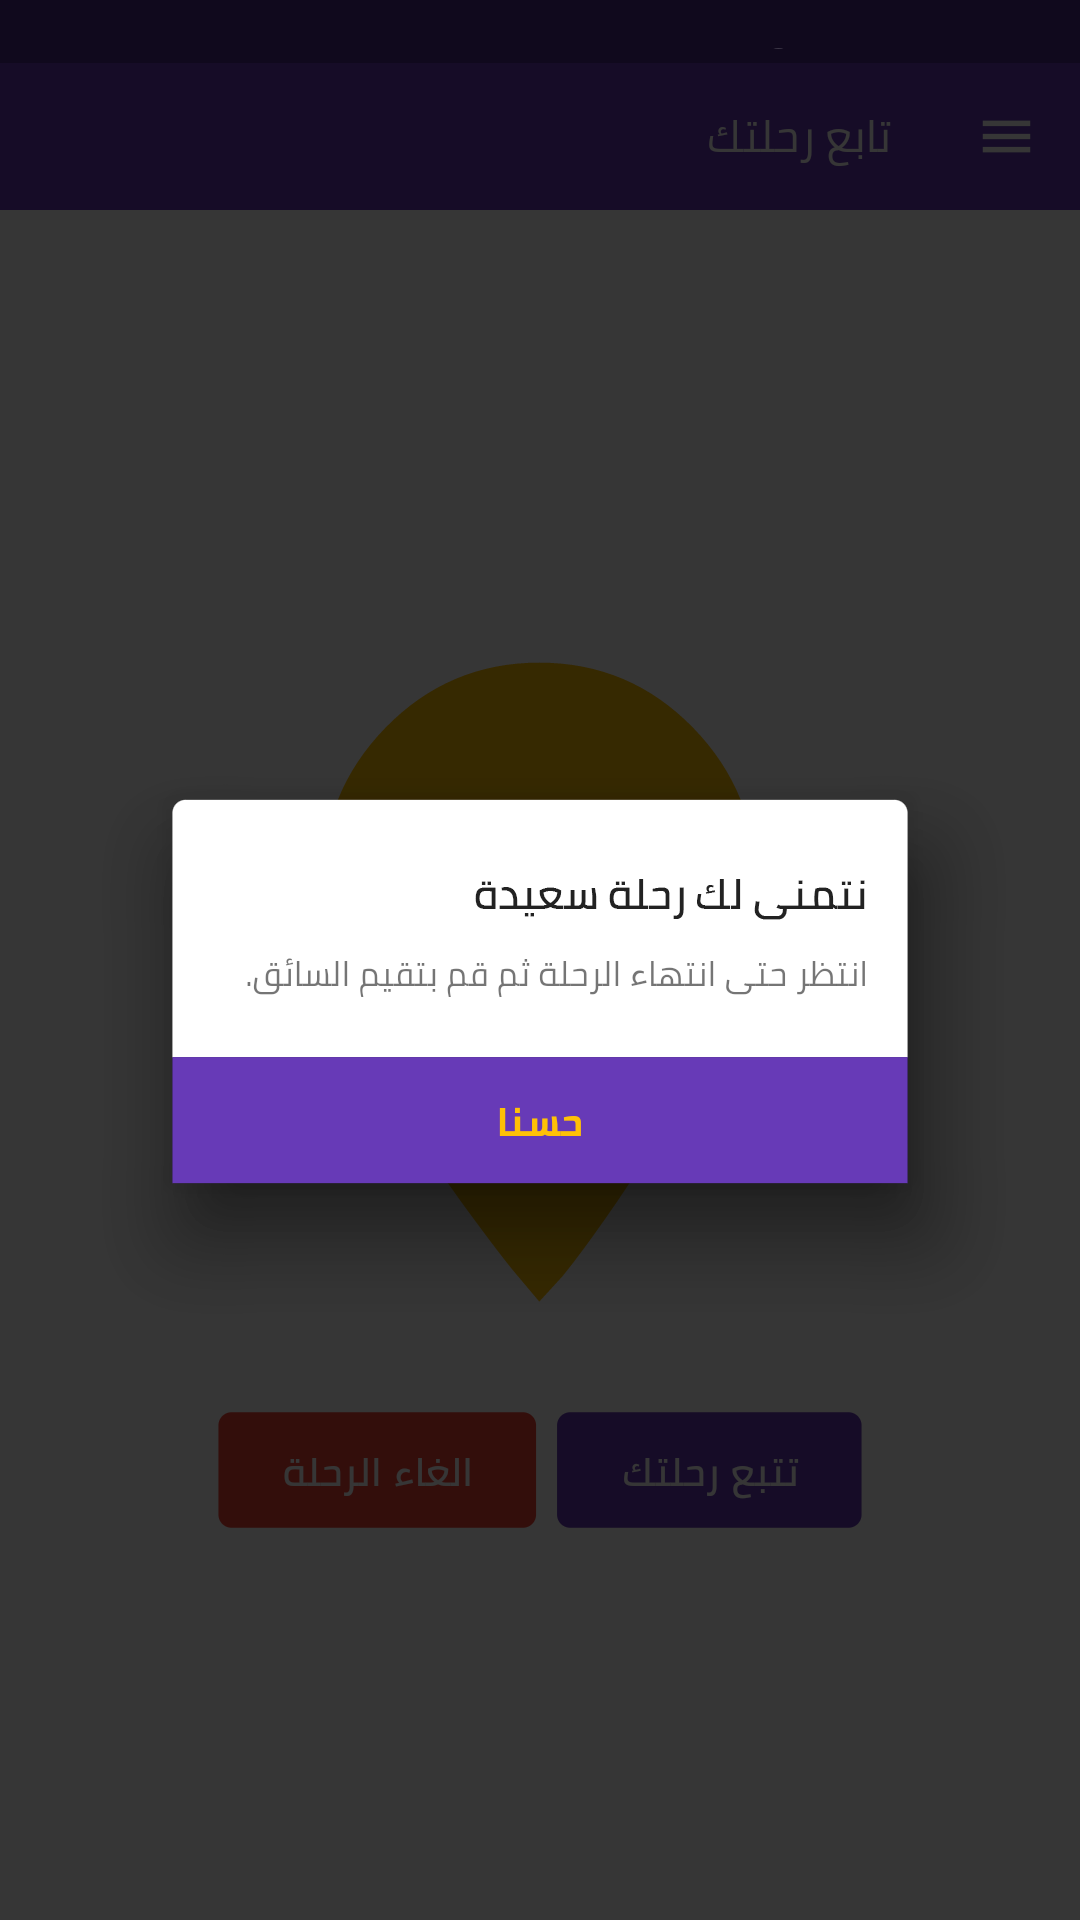
\includegraphics[width=0.5\linewidth]{images/ch3/8.png} 
    
    \label{fig7:d} 
  \end{subfigure} 
  \caption{ Tracking page}
  \label{fig7} 
\end{figure}

\begin{figure}[H] 
  \begin{subfigure}[b]{0.5\linewidth}
    \centering
    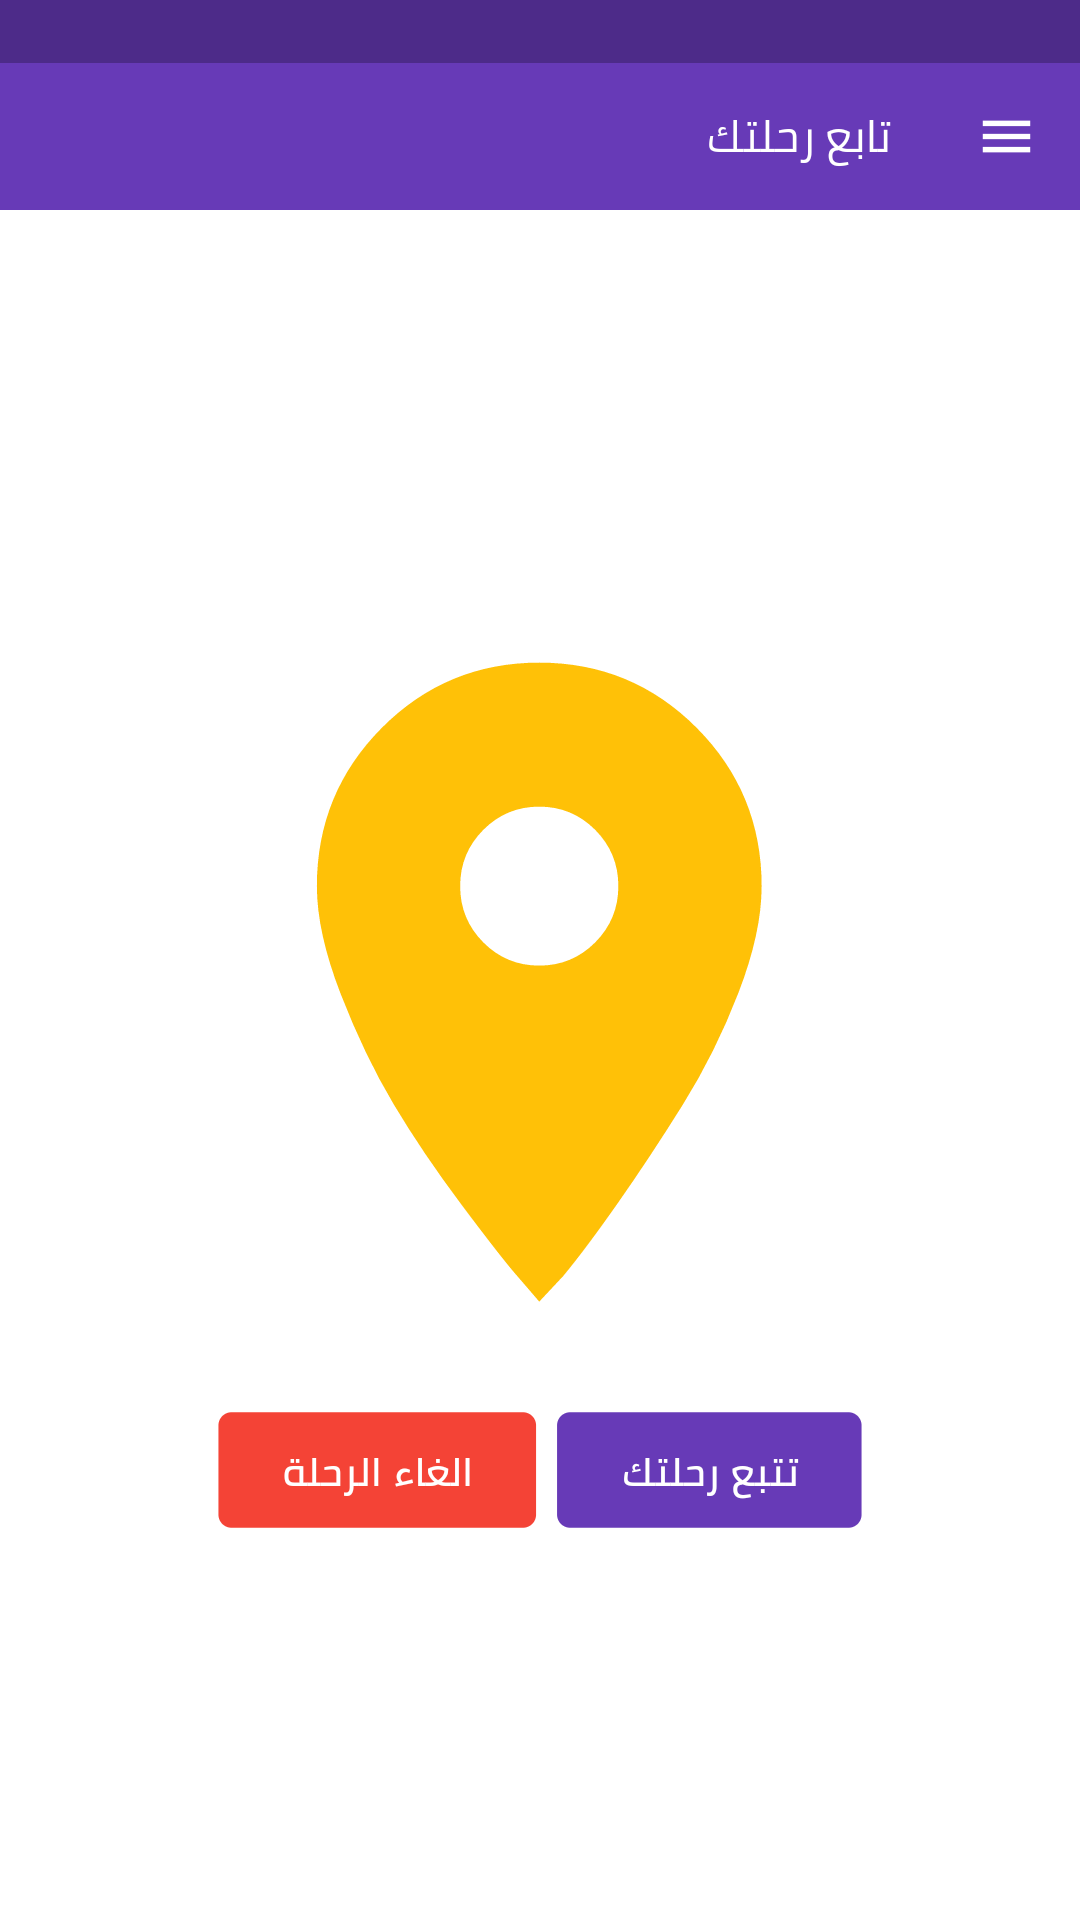
\includegraphics[width=0.5\linewidth]{images/ch3/9.png}
  
    \label{fig7:c} 
  \end{subfigure}%% 
  \begin{subfigure}[b]{0.5\linewidth}
    \centering
    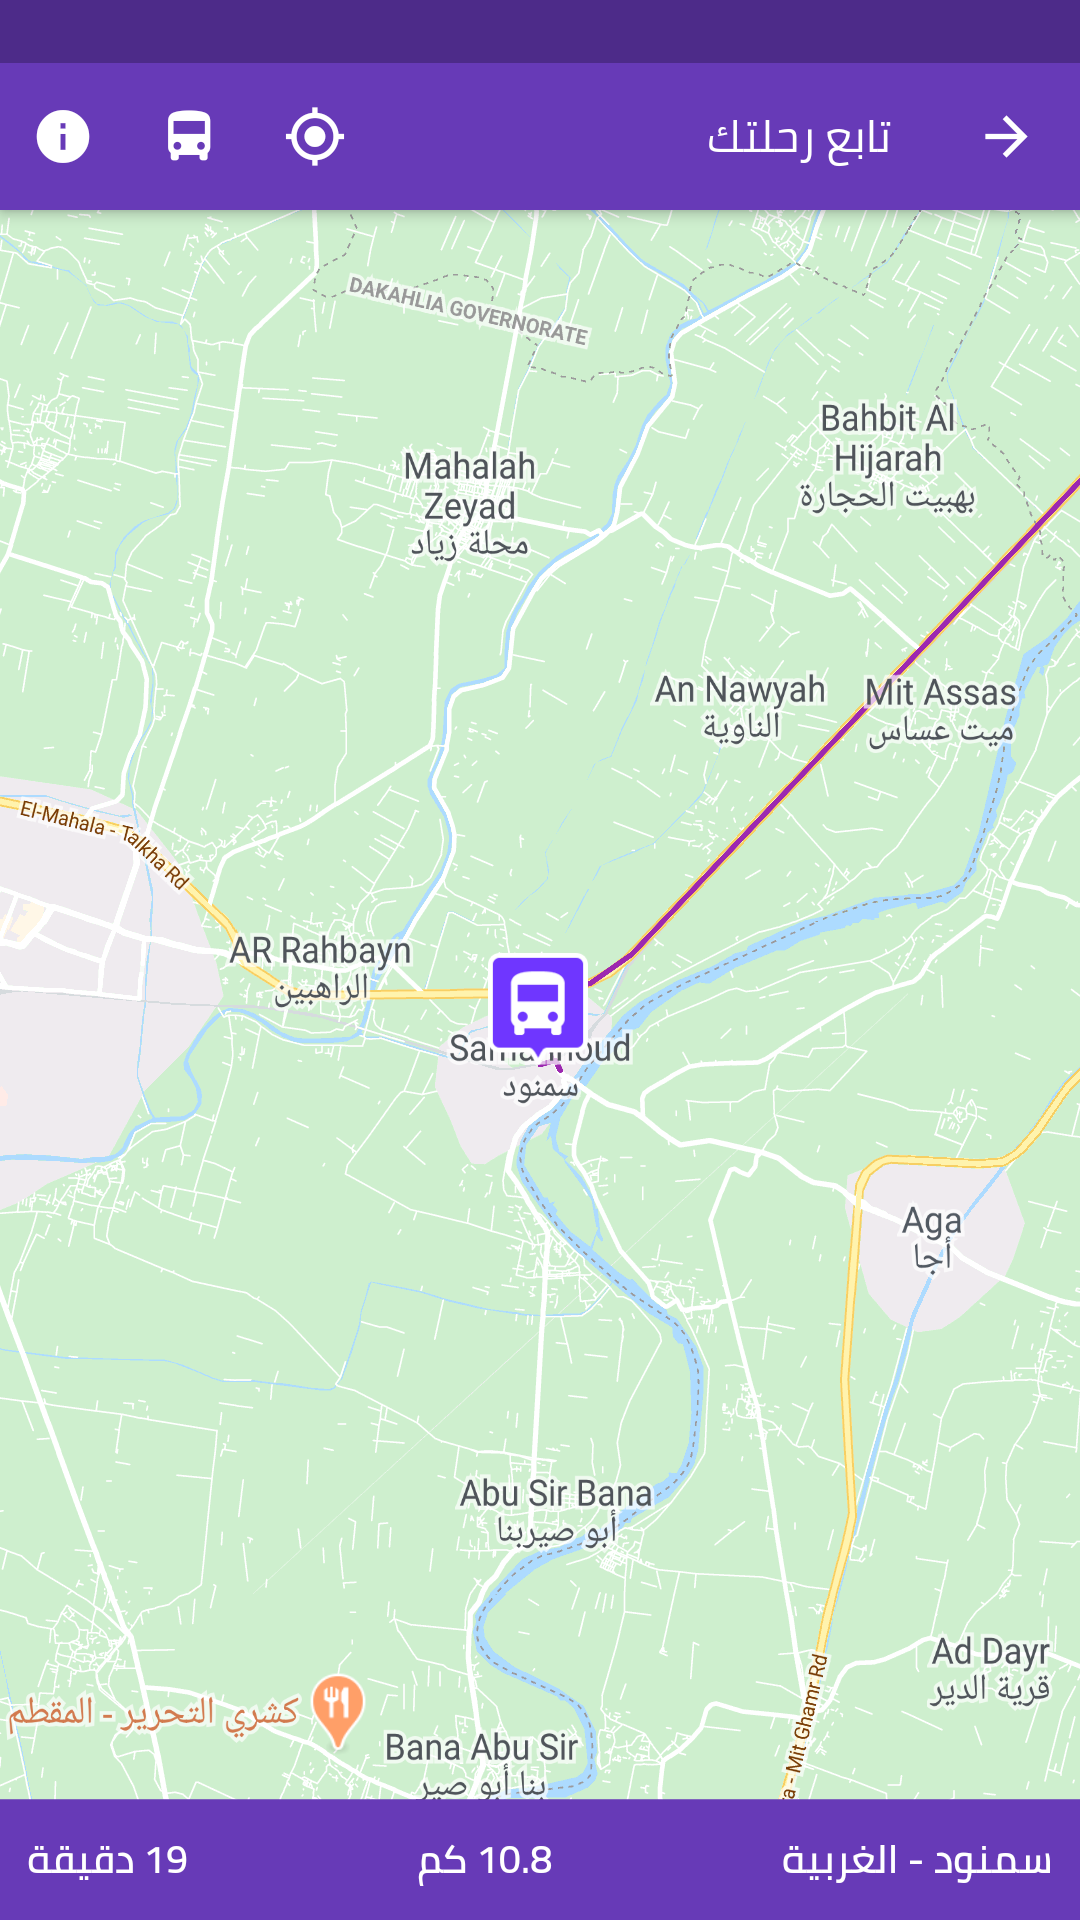
\includegraphics[width=0.5\linewidth]{images/ch3/10.png} 
    \label{fig7:d} 
  \end{subfigure} 
  \begin{subfigure}[b]{0.5\linewidth}
    \centering
    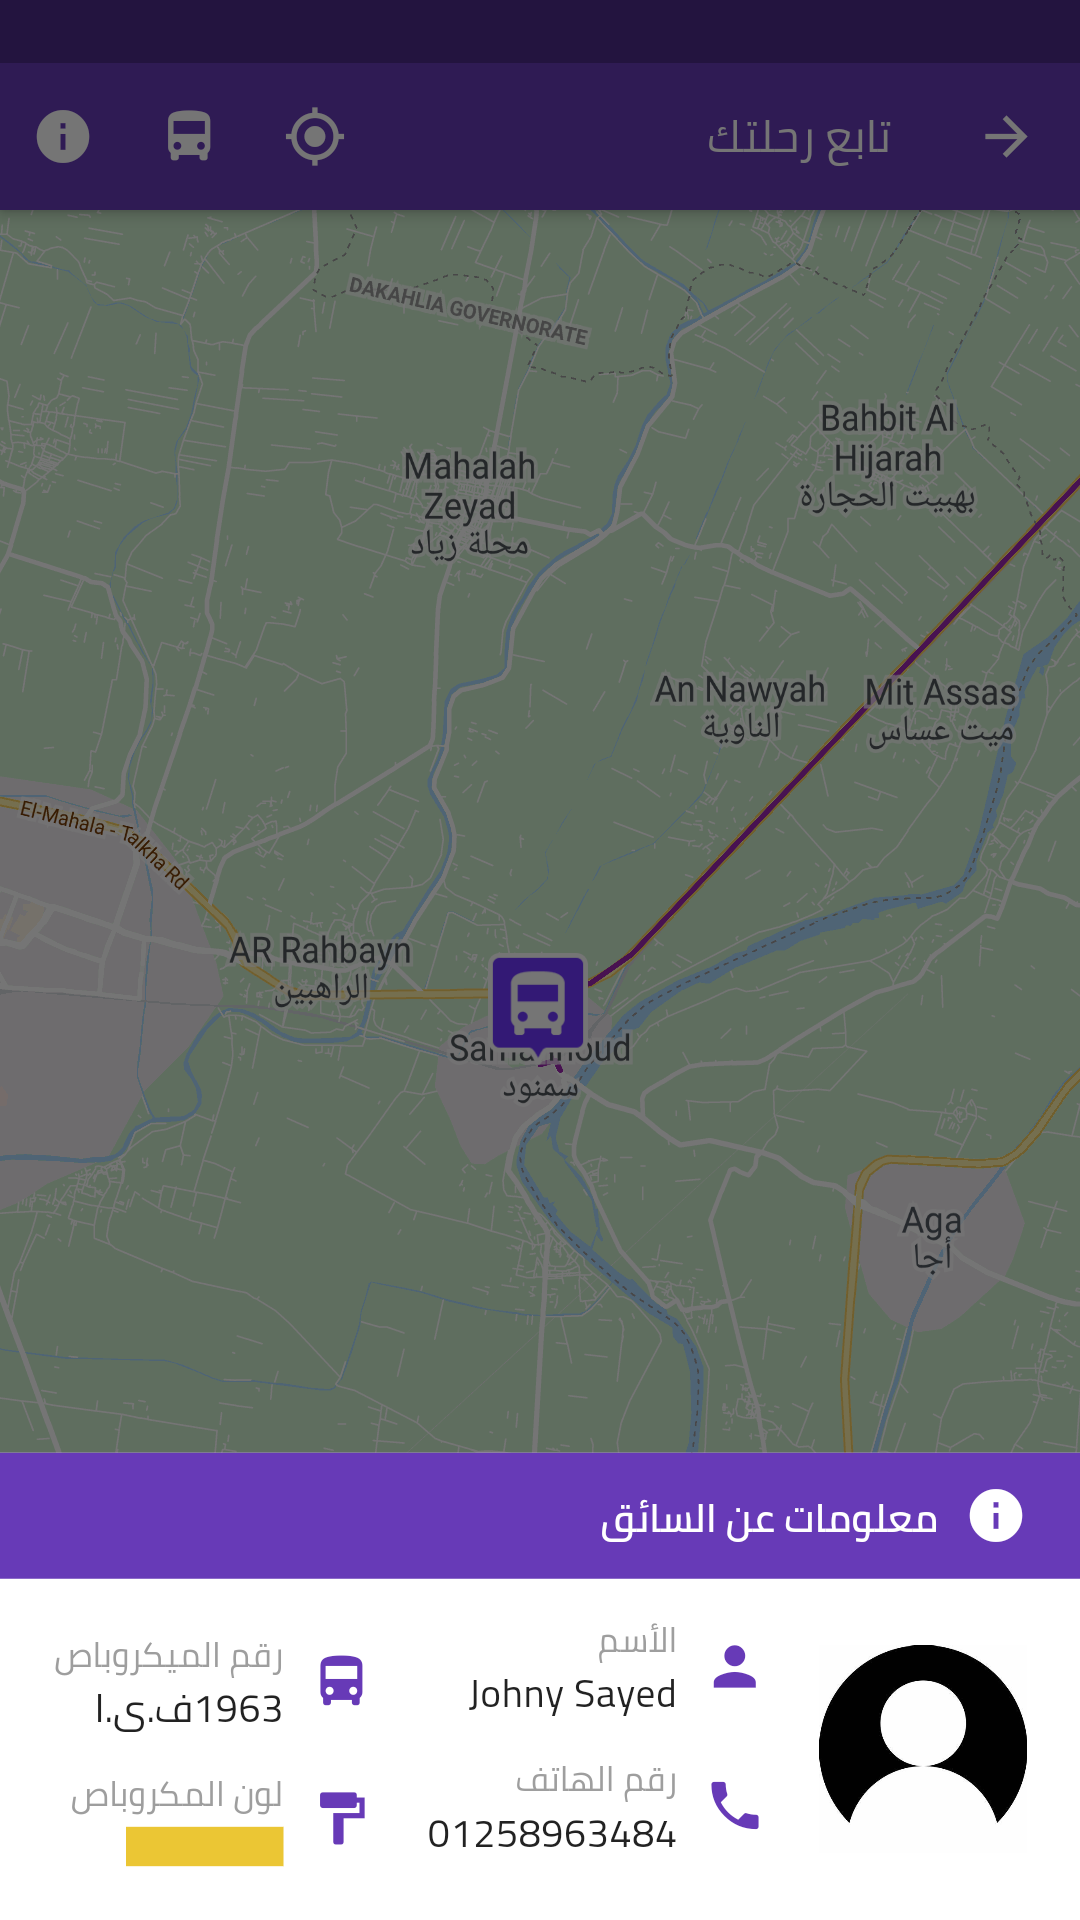
\includegraphics[width=0.5\linewidth]{images/ch3/11.png}
  
    \label{fig7:c} 
  \end{subfigure}%% 
  \begin{subfigure}[b]{0.5\linewidth}
    \centering
    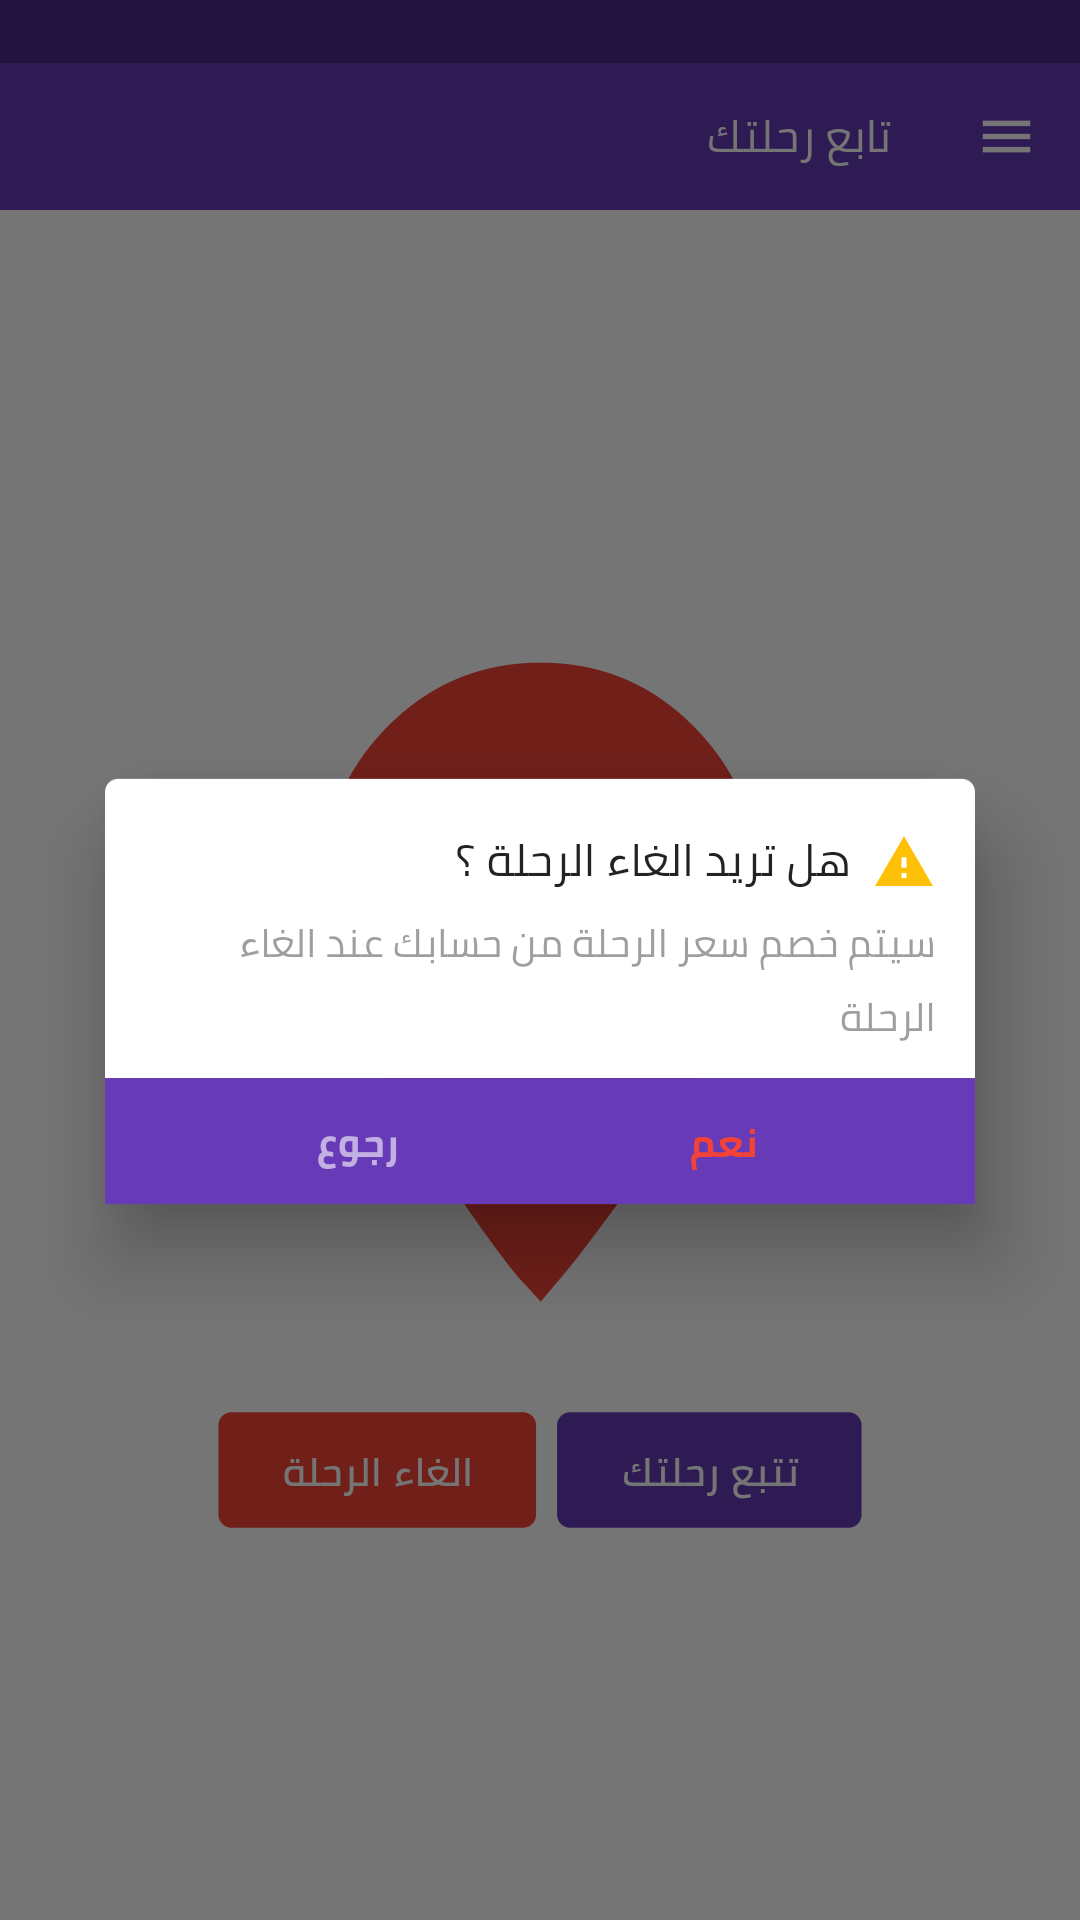
\includegraphics[width=0.5\linewidth]{images/ch3/7. Cancel.png}
  
    \label{fig7:c} 
  \end{subfigure}%% 
  \caption{ Tracking page}
  \label{fig7} 
\end{figure}
\newpage
\par \textbf{\textit{Rating Page:}}  for both the driver and the user can evaluate their ride and this appears after the end of each ride
\begin{figure}[H]
    \centering
    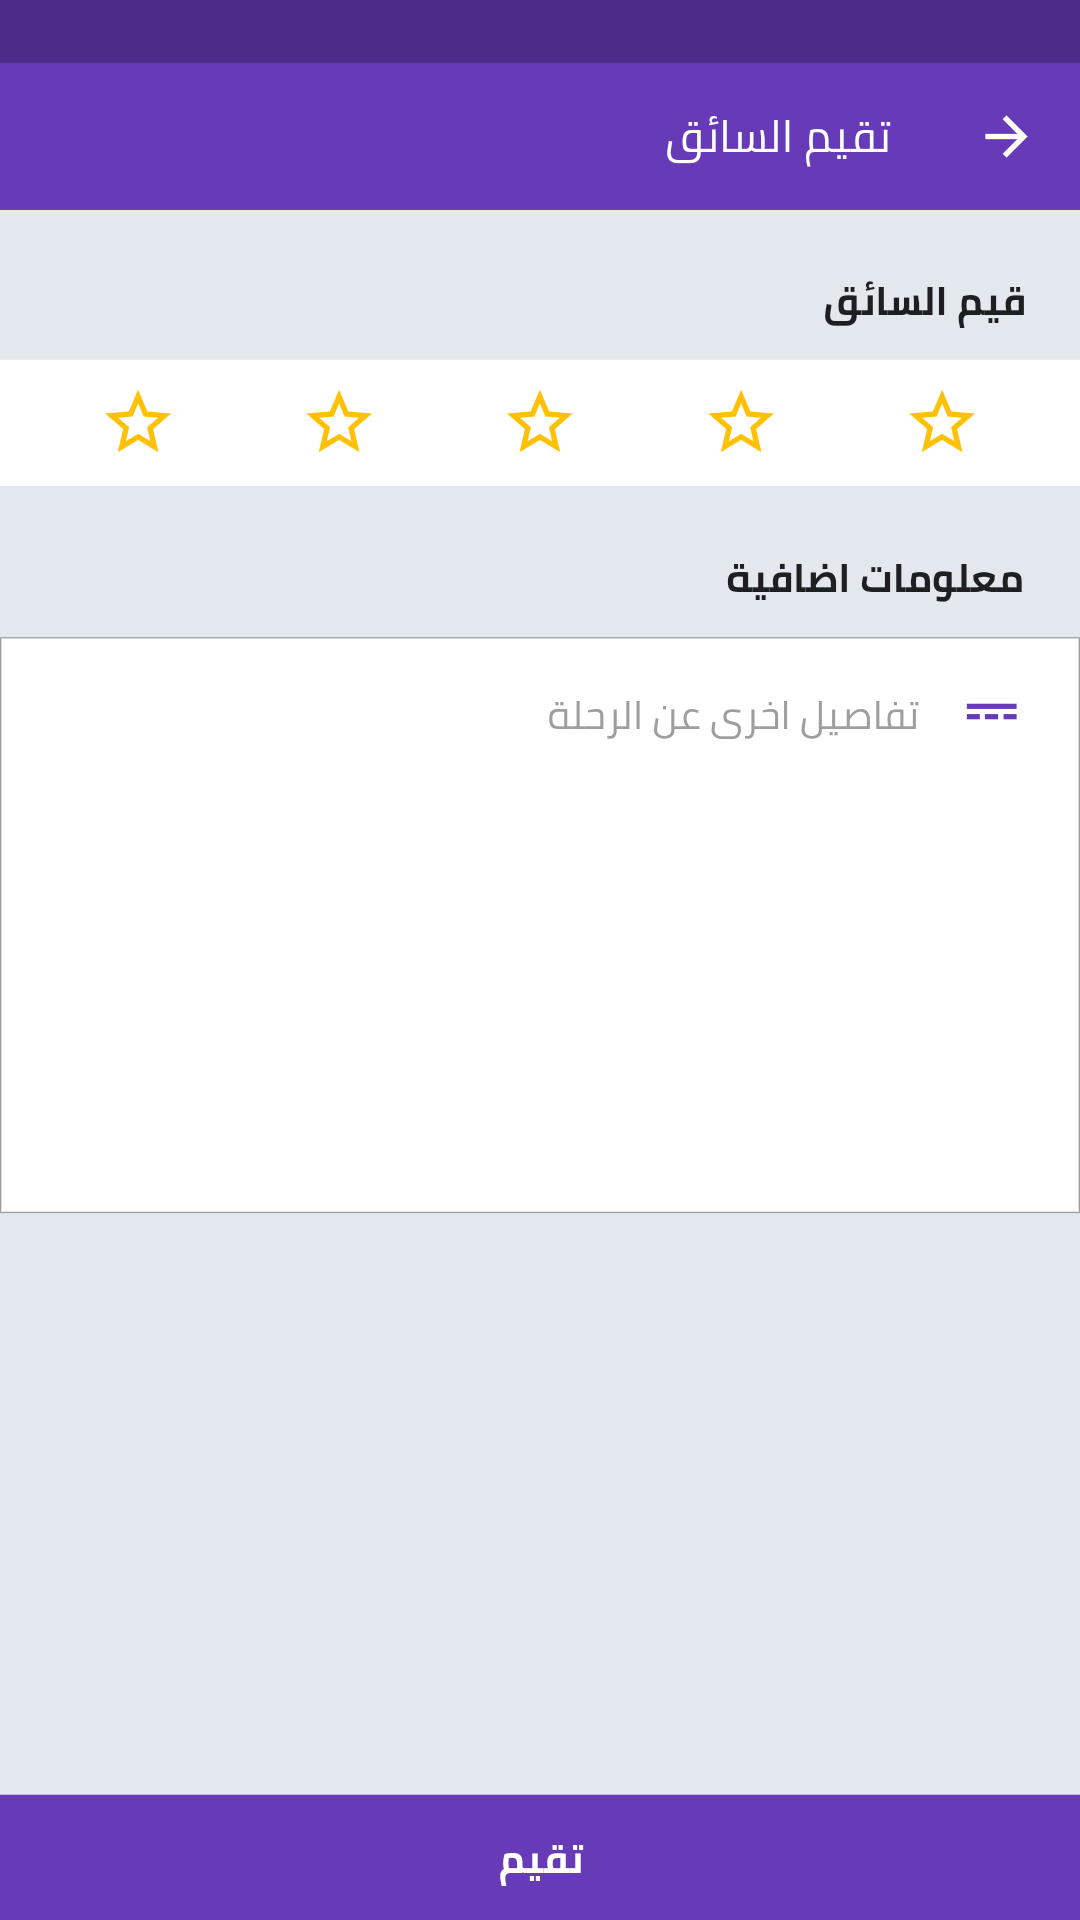
\includegraphics[width=0.3\linewidth]{images/ch3/12.png}
    \caption{Rating Page}
    \label{fig:my_label}
\end{figure}
\par  \textbf{\textit{Profile Page:}}
\begin{figure}[H] 
      \centering

  \begin{subfigure}[b]{0.5\linewidth}
    \centering
    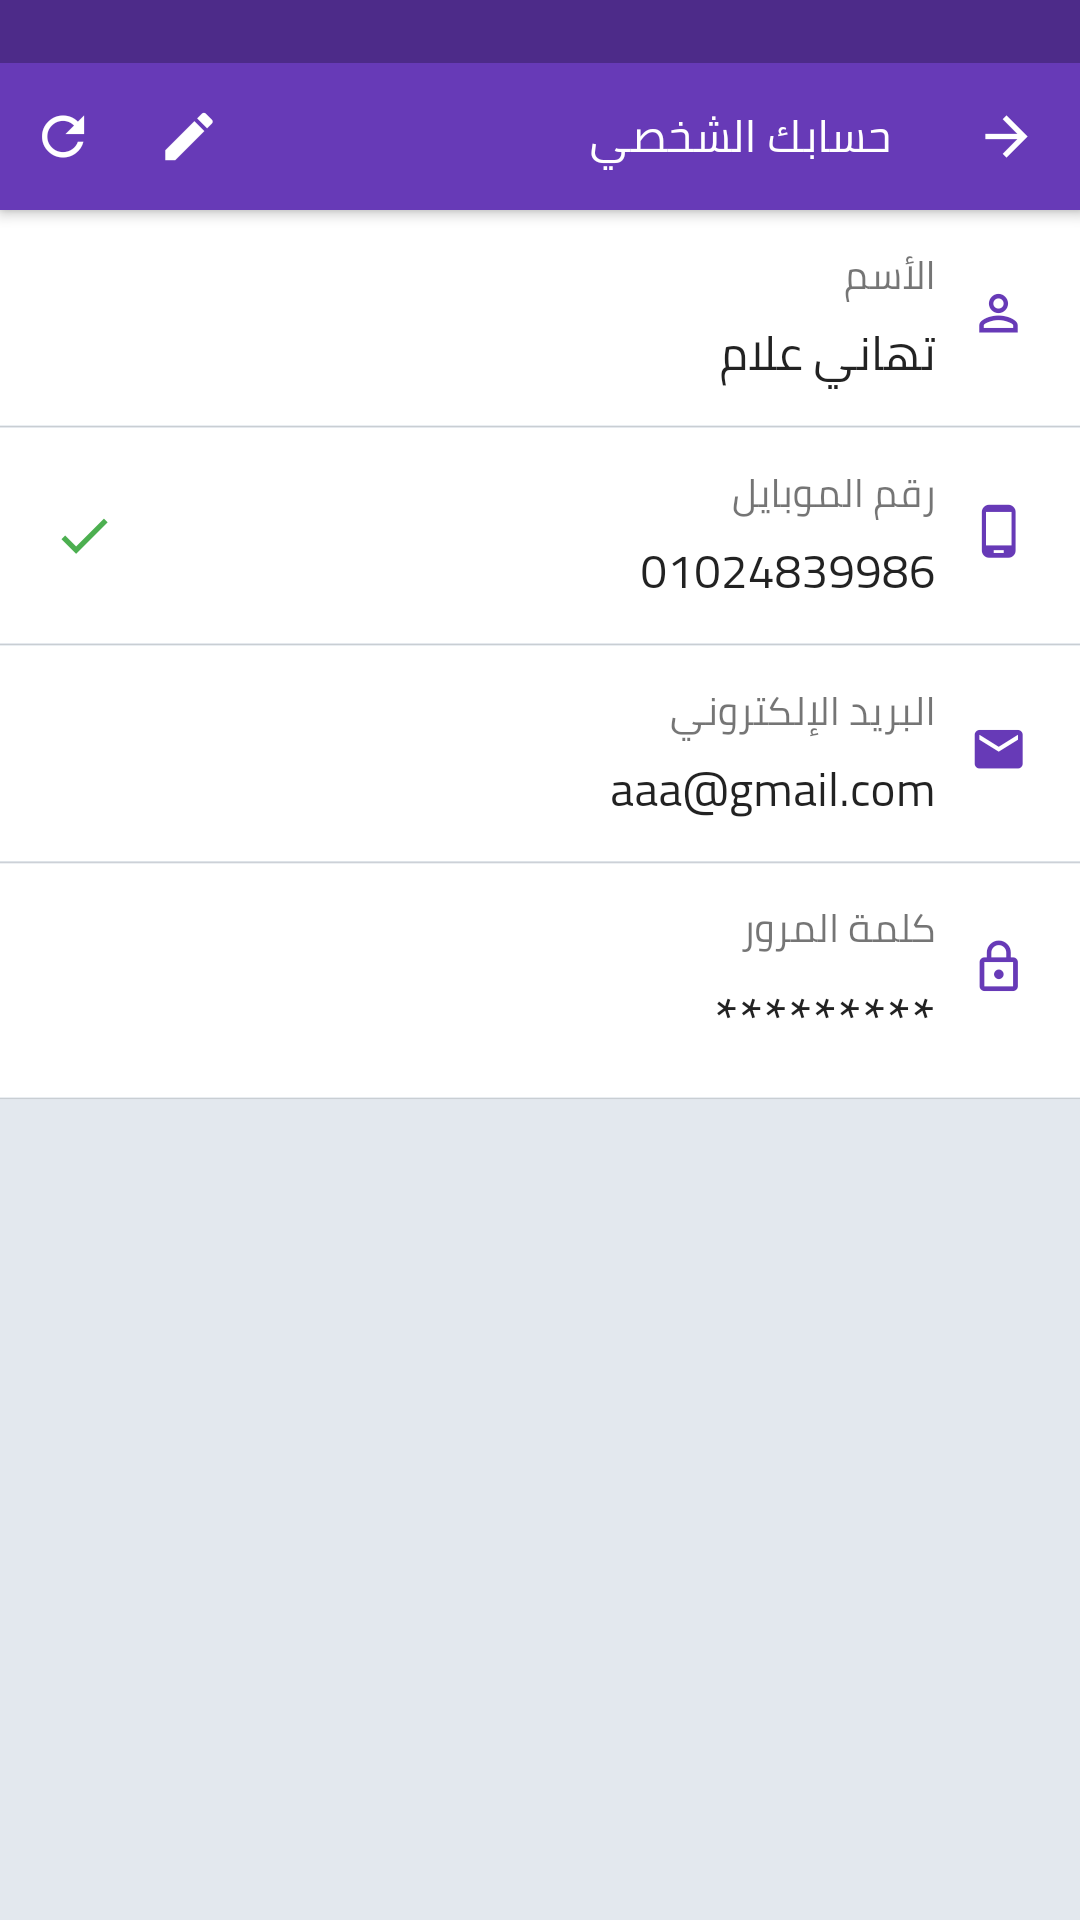
\includegraphics[width=0.5\linewidth]{images/ch3/Profile/0.png}
  
    \label{fig7:c} 
  \end{subfigure}%% 
      \caption{Profile page}

  \label{fig7} 
\end{figure}

\begin{figure}[H] 
  
  \begin{subfigure}[b]{0.5\linewidth}
    \centering
    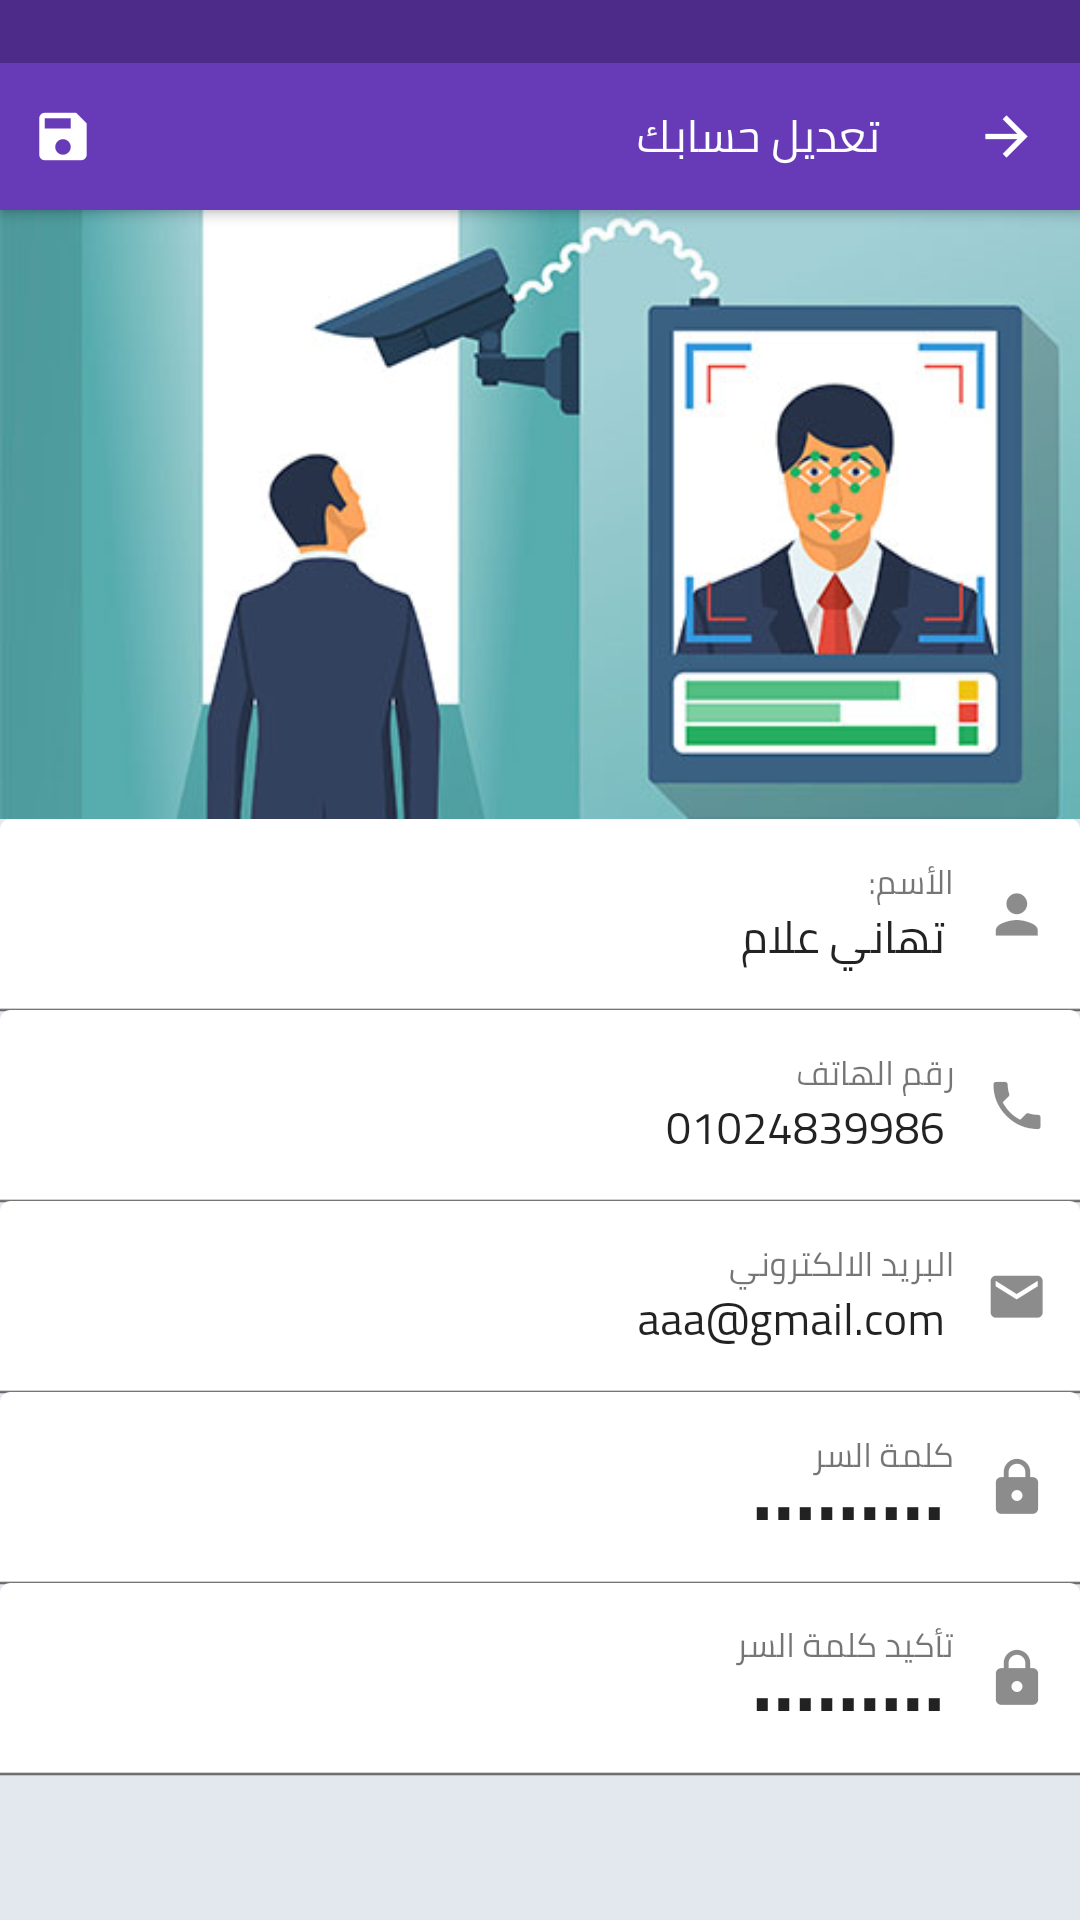
\includegraphics[width=0.5\linewidth]{images/ch3/Profile/1.png}
  
    \label{fig7:a} 
  \end{subfigure}%% 
    \begin{subfigure}[b]{0.5\linewidth}
    \centering
    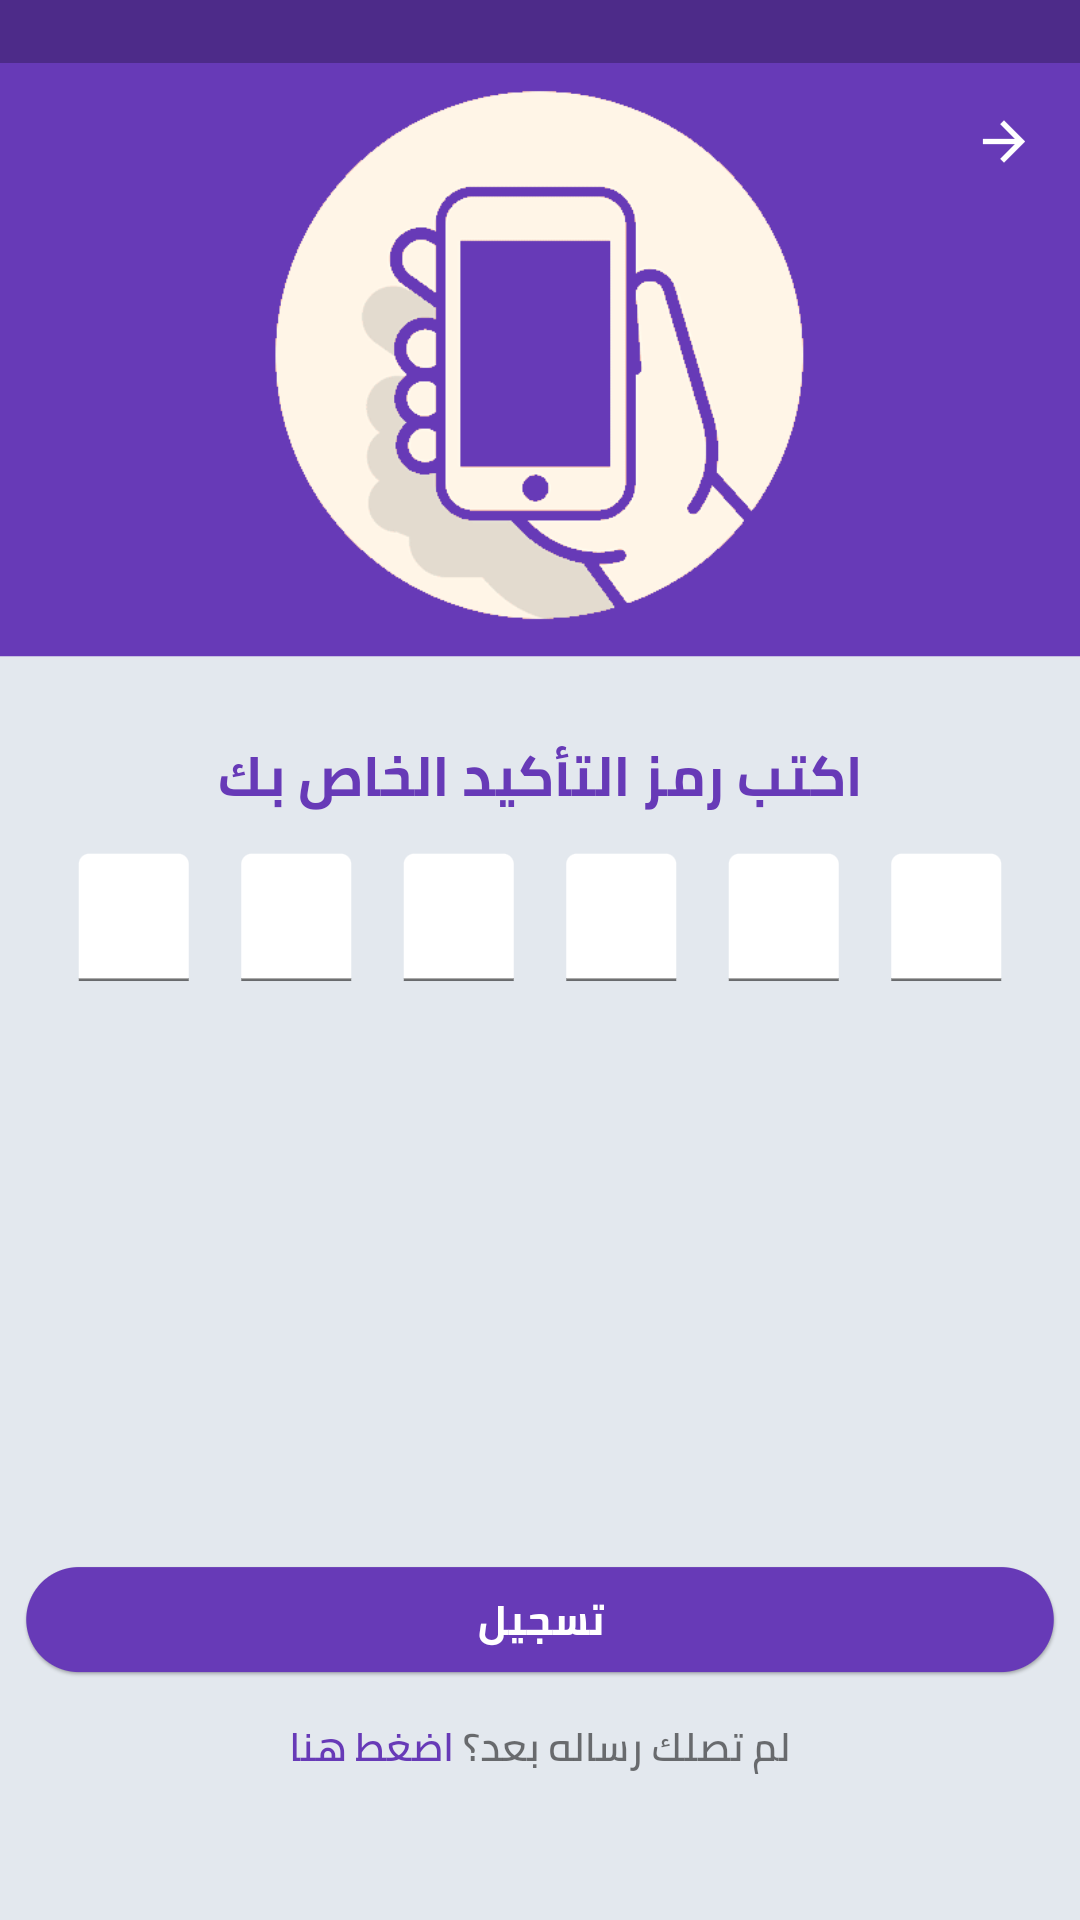
\includegraphics[width=0.5\linewidth]{images/ch3/Profile/2.png}
  
    \label{fig7:b} 
  \end{subfigure}%% 
  \caption{ Editing profile page}
  \label{fig7} 
\end{figure}


\par  \textbf{\textit{Family services Page:}}

\begin{figure}[H] 
  
  \begin{subfigure}[b]{0.5\linewidth}
    \centering
    
\includegraphics[width=0.5\linewidth]{images/ch3/family/0.png}
  
    \label{fig7:a} 
  \end{subfigure}%% 
    \begin{subfigure}[b]{0.5\linewidth}
    \centering
    
\includegraphics[width=0.5\linewidth]{images/ch3/family/1.png}
  
    \label{fig7:b} 
  \end{subfigure}%% 
  \caption{ Family services Page}
  \label{fig7} 
\end{figure}
\begin{figure}[H] 
  
  \begin{subfigure}[b]{0.5\linewidth}
    \centering
    
\includegraphics[width=0.5\linewidth]{images/ch3/family/2.png}
  
    \label{fig7:c} 
  \end{subfigure}%% 
    \begin{subfigure}[b]{0.5\linewidth}
    \centering
    
\includegraphics[width=0.5\linewidth]{images/ch3/family/3.png}
  
    \label{fig7:d} 
  \end{subfigure}%% 
    \begin{subfigure}[b]{0.5\linewidth}
    \centering
    
\includegraphics[width=0.5\linewidth]{images/ch3/family/4.png}
  
    \label{fig7:e} 
  \end{subfigure}%% 
  \label{fig7} 
\end{figure}
\begin{figure}[H] 
  
    \begin{subfigure}[b]{0.5\linewidth}
    \centering
    
\includegraphics[width=0.5\linewidth]{images/ch3/family/6.png}
  
  \end{subfigure}%% 
    \begin{subfigure}[b]{0.5\linewidth}
    \centering
    
\includegraphics[width=0.5\linewidth]{images/ch3/family/7.png}
  
  \end{subfigure}%
  \par\par
  \begin{itemize}
  \item The application provides for users Family services which can make an invitation for someone who uses the app
\end{itemize}


  
  \label{fig7} 
\end{figure}
\begin{figure}[H] 
 \begin{subfigure}[b]{0.5\linewidth}
    \centering
    
\includegraphics[width=0.5\linewidth]{images/ch3/family/8.png}
  
  \end{subfigure}%% 
    \begin{subfigure}[b]{0.5\linewidth}
    \centering
    
\includegraphics[width=0.5\linewidth]{images/ch3/family/9.png}
  
  \end{subfigure}%% 
    \begin{subfigure}[b]{0.5\linewidth}
    \centering
    
\includegraphics[width=0.5\linewidth]{images/ch3/family/10.png}
  
  \end{subfigure}%%
    \caption{ Family services Page}

  \end{figure}
  
 \par\textbf{\textit{Payment Page:}} \par
 It allows the user to use his own balance for the payment process, the ability to transfer money and borrow some money too.
 \begin{figure}[H] 
 \begin{subfigure}[b]{0.5\linewidth}
    \centering
    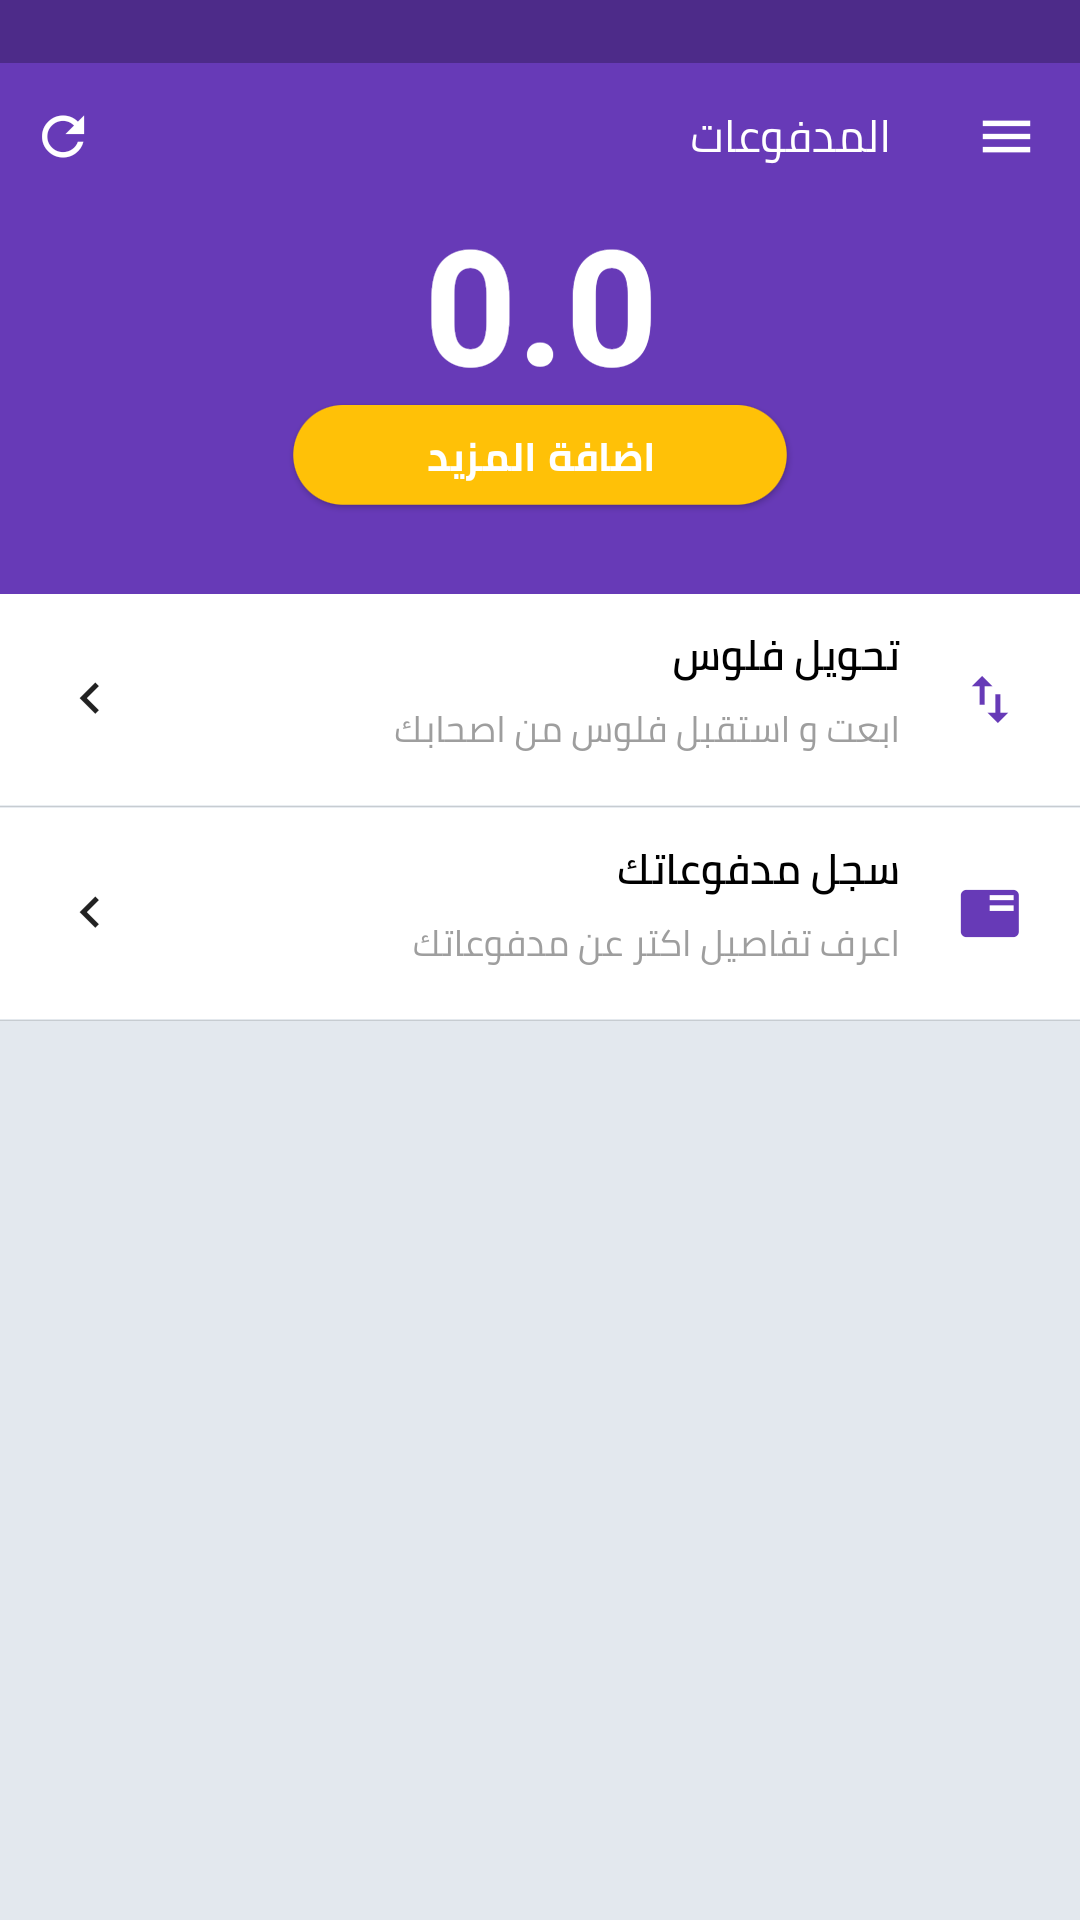
\includegraphics[width=0.5\linewidth]{images/ch3/payment/Adding Credit/0.png}
  
  \end{subfigure}%% 
    \begin{subfigure}[b]{0.5\linewidth}
    \centering
    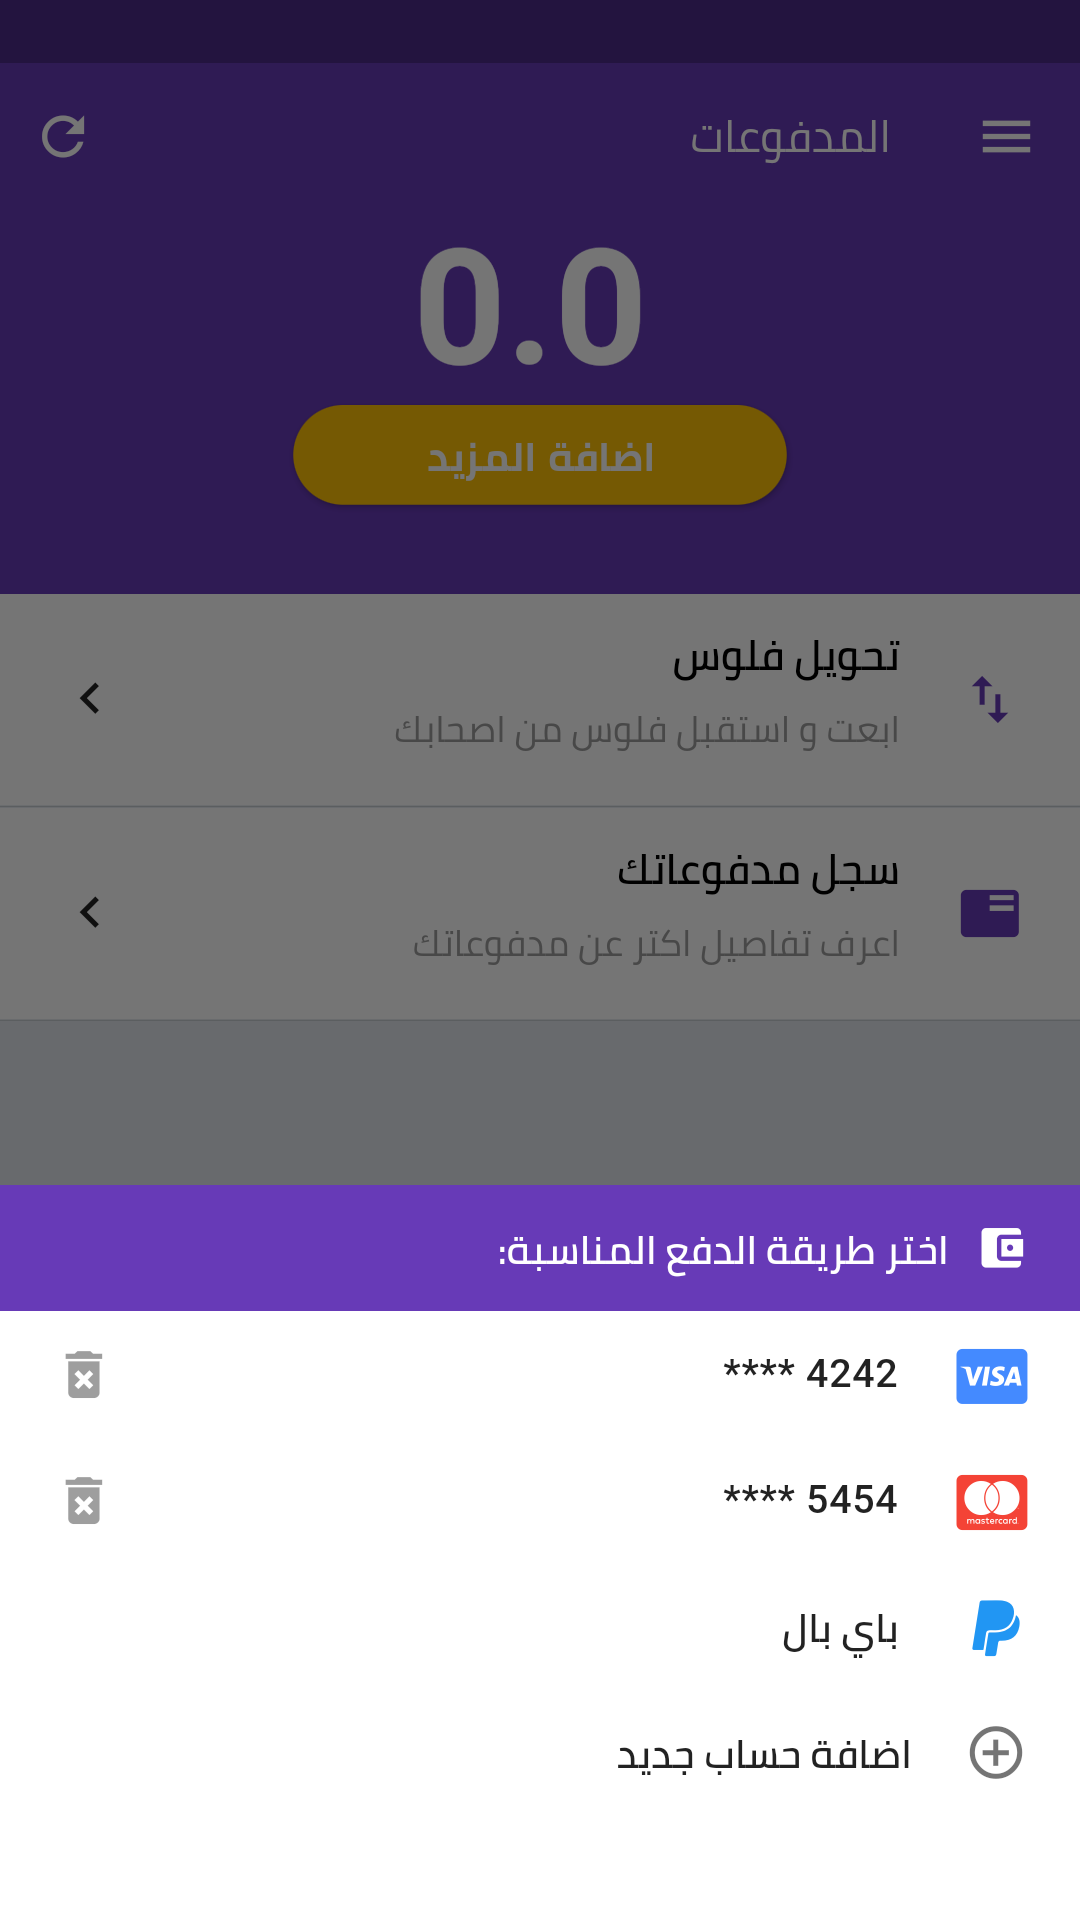
\includegraphics[width=0.5\linewidth]{images/ch3/payment/Adding Credit/1.png}
  
  \end{subfigure}%% 

    \caption{ Add credit Page}

  \end{figure}
  
  \begin{figure}[H] 
 \begin{subfigure}[b]{0.5\linewidth}
    \centering
    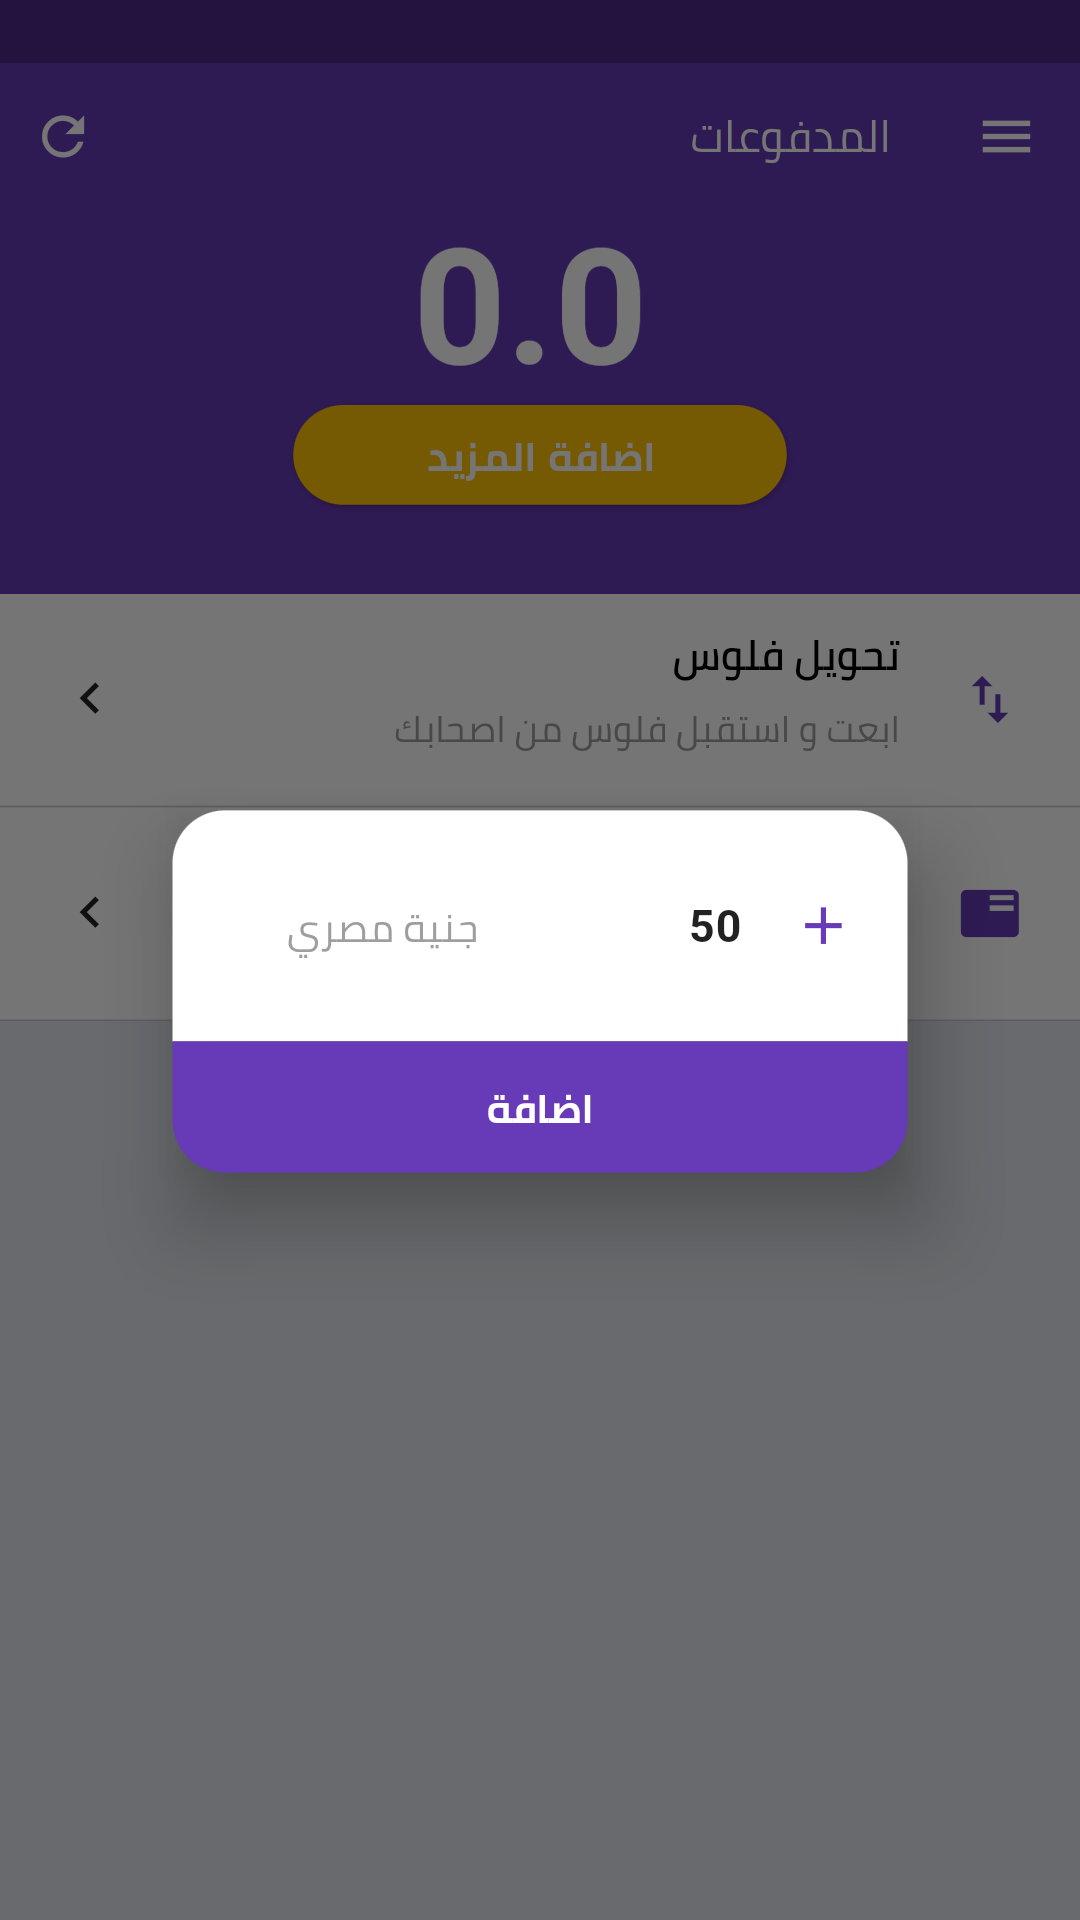
\includegraphics[width=0.5\linewidth]{images/ch3/payment/Adding Credit/2.png}
  
  \end{subfigure}%%
    \begin{subfigure}[b]{0.5\linewidth}
    \centering
    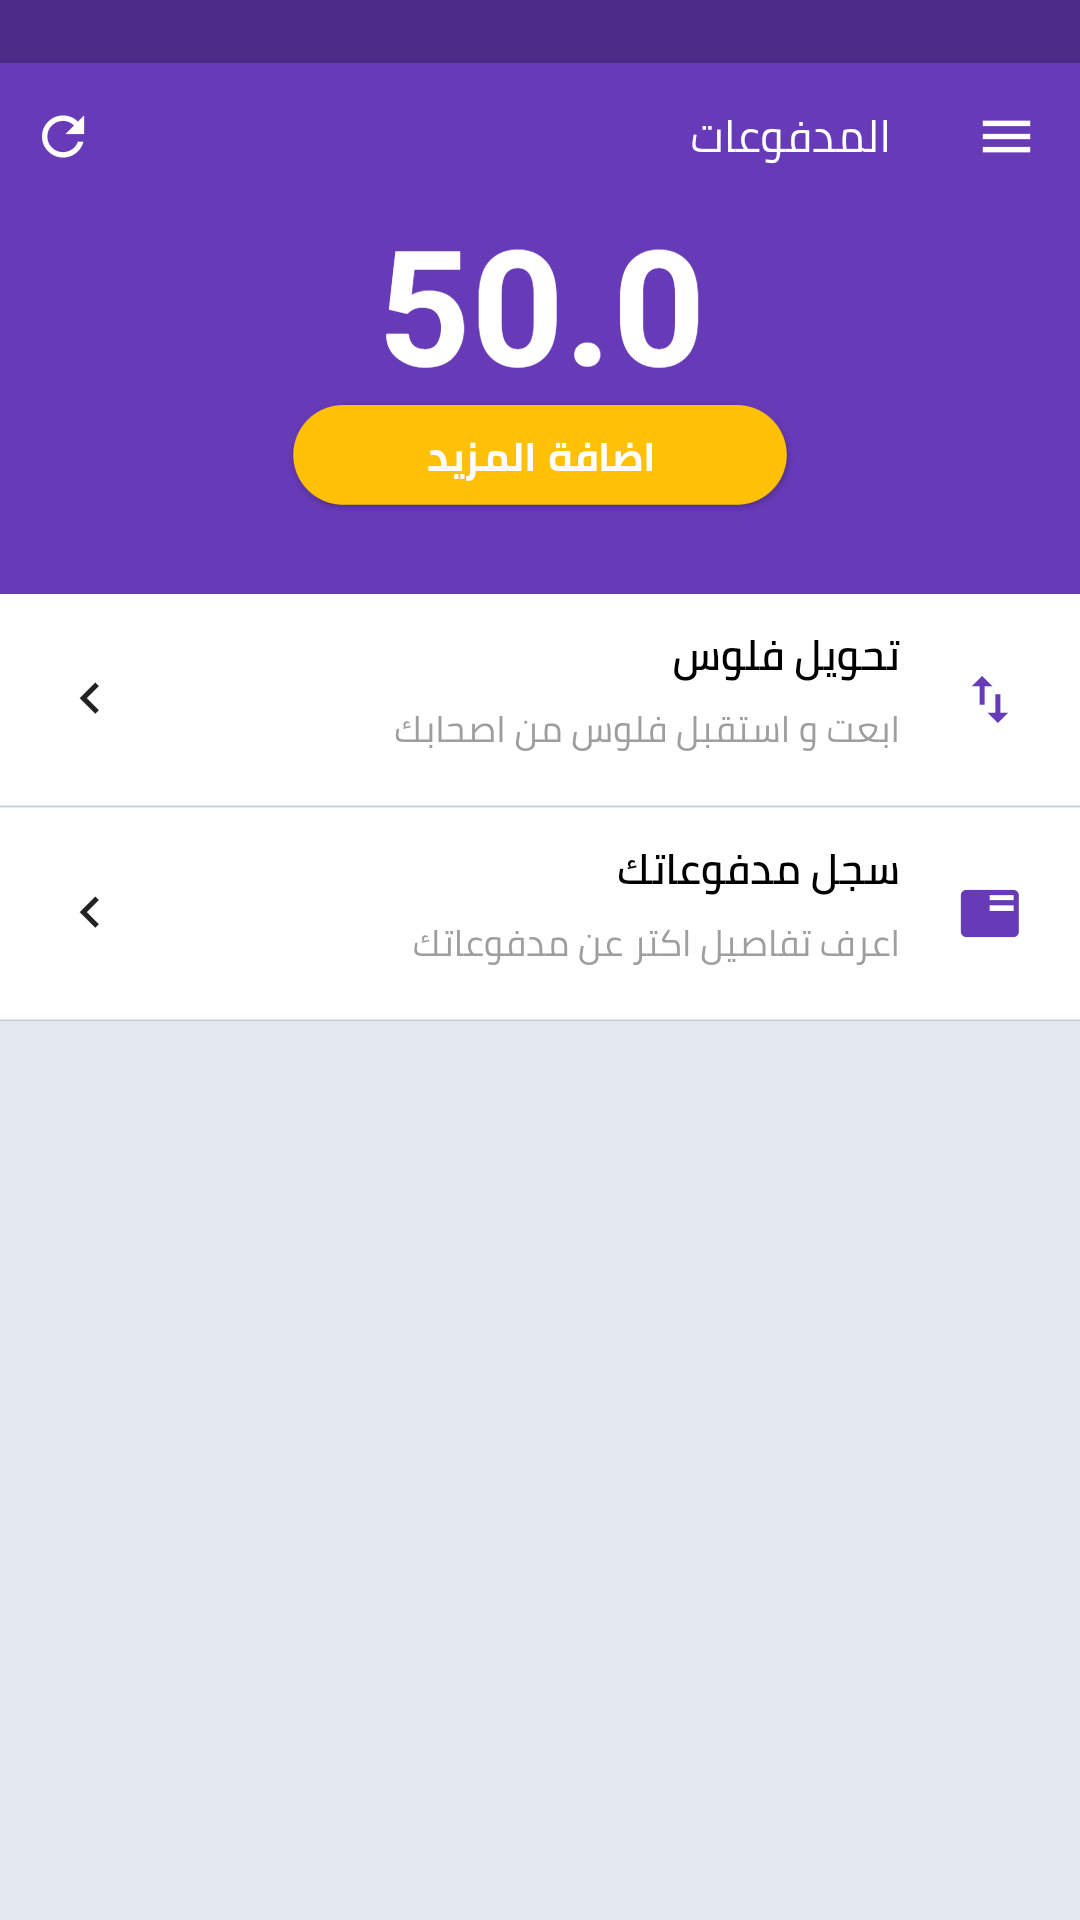
\includegraphics[width=0.5\linewidth]{images/ch3/payment/Adding Credit/3.png}
  
  \end{subfigure}%% 
    \caption{ Payment services history Page}

  \end{figure}

    \begin{figure}[H] 

    \begin{subfigure}[b]{0.5\linewidth}
    \centering
    
\includegraphics[width=0.5\linewidth]{images/ch3/payment/Adding Credit/4.png}
  \end{subfigure}%%
   \begin{subfigure}[b]{0.5\linewidth}
    \centering
    
\includegraphics[width=0.5\linewidth]{images/ch3/payment/Adding Credit/5.png}
  
  \end{subfigure}%%
    \caption{ Payment services Page}

  \end{figure}
      \begin{figure}[H] 

    \begin{subfigure}[b]{0.5\linewidth}
    \centering
    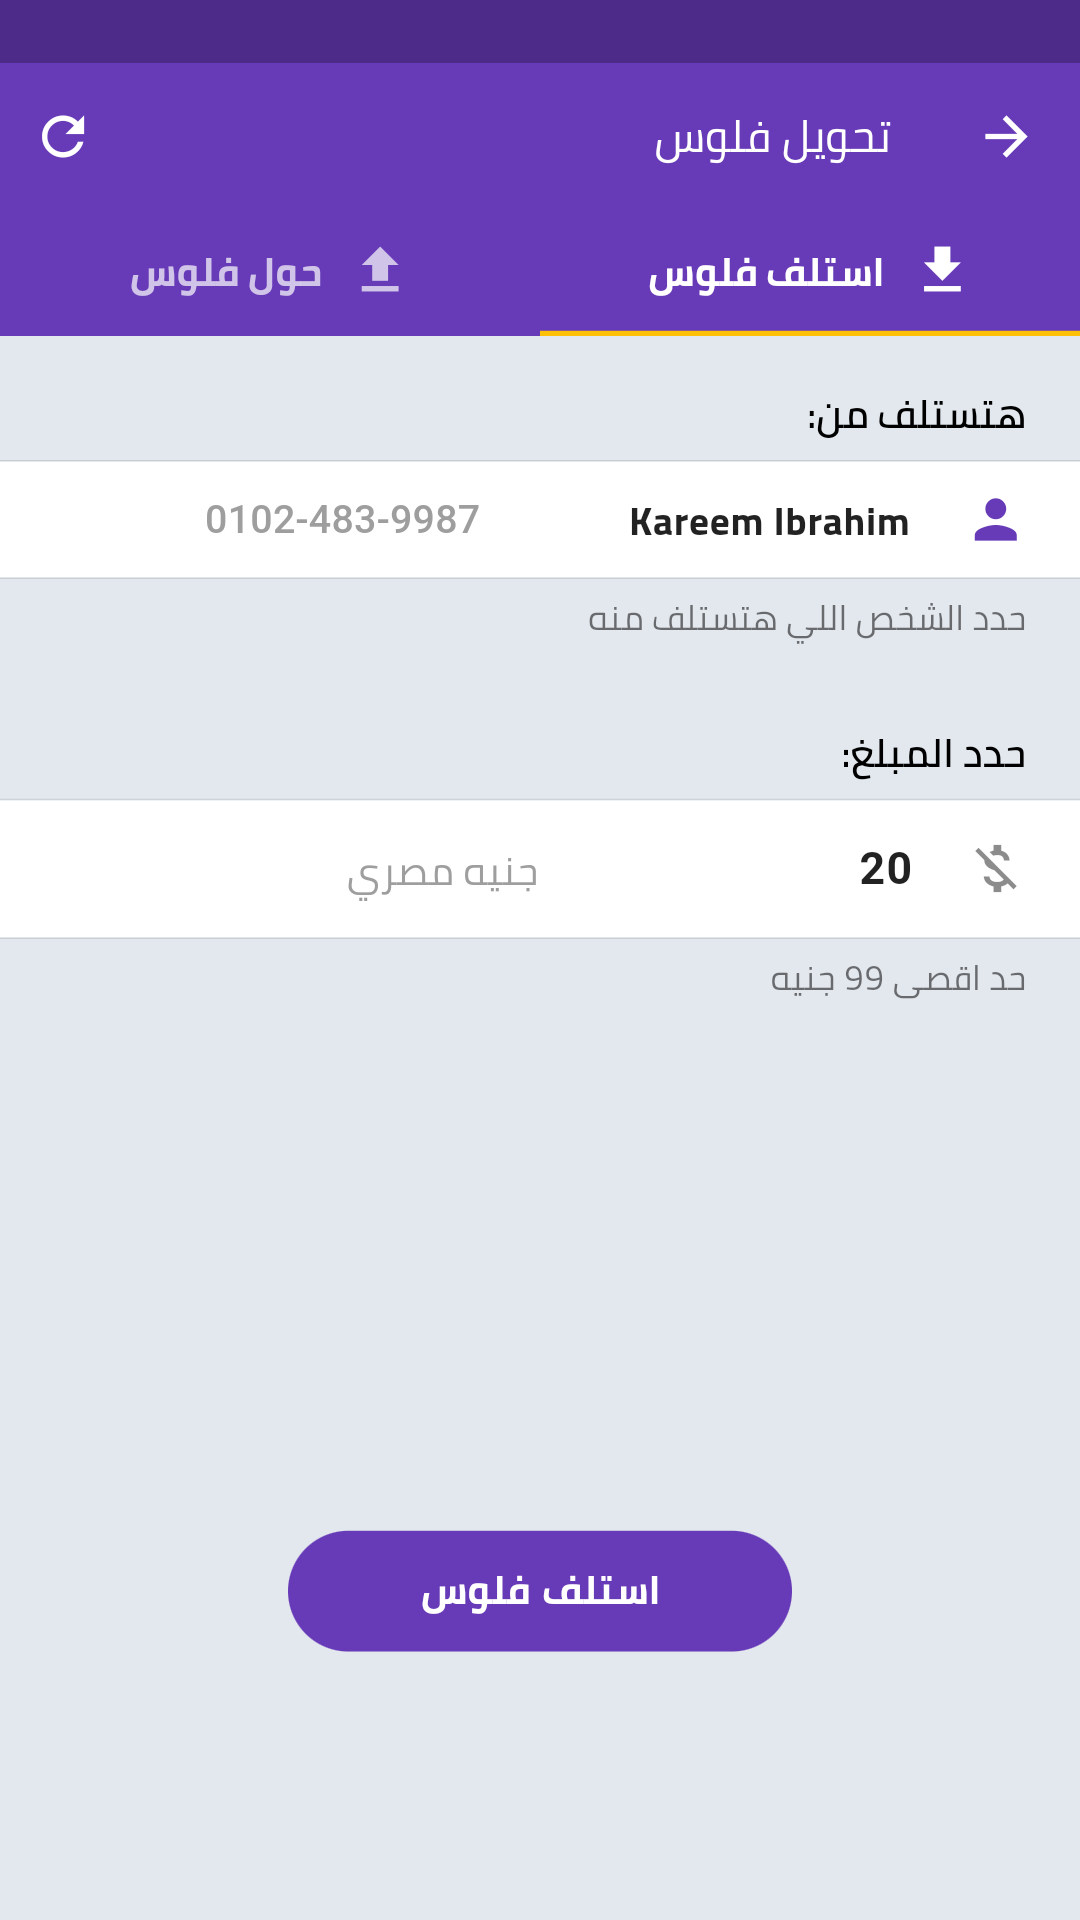
\includegraphics[width=0.5\linewidth]{images/ch3/payment/Loaning/1.png}
  
  \end{subfigure}%%
   \begin{subfigure}[b]{0.5\linewidth}
    \centering
    
\includegraphics[width=0.5\linewidth]{images/ch3/payment/Loaning/7.png}
  
  \end{subfigure}%%
    \caption{Transfer and borrow money Page}

  \end{figure}
        \begin{figure}[H] 

    \begin{subfigure}[b]{0.5\linewidth}
    \centering
    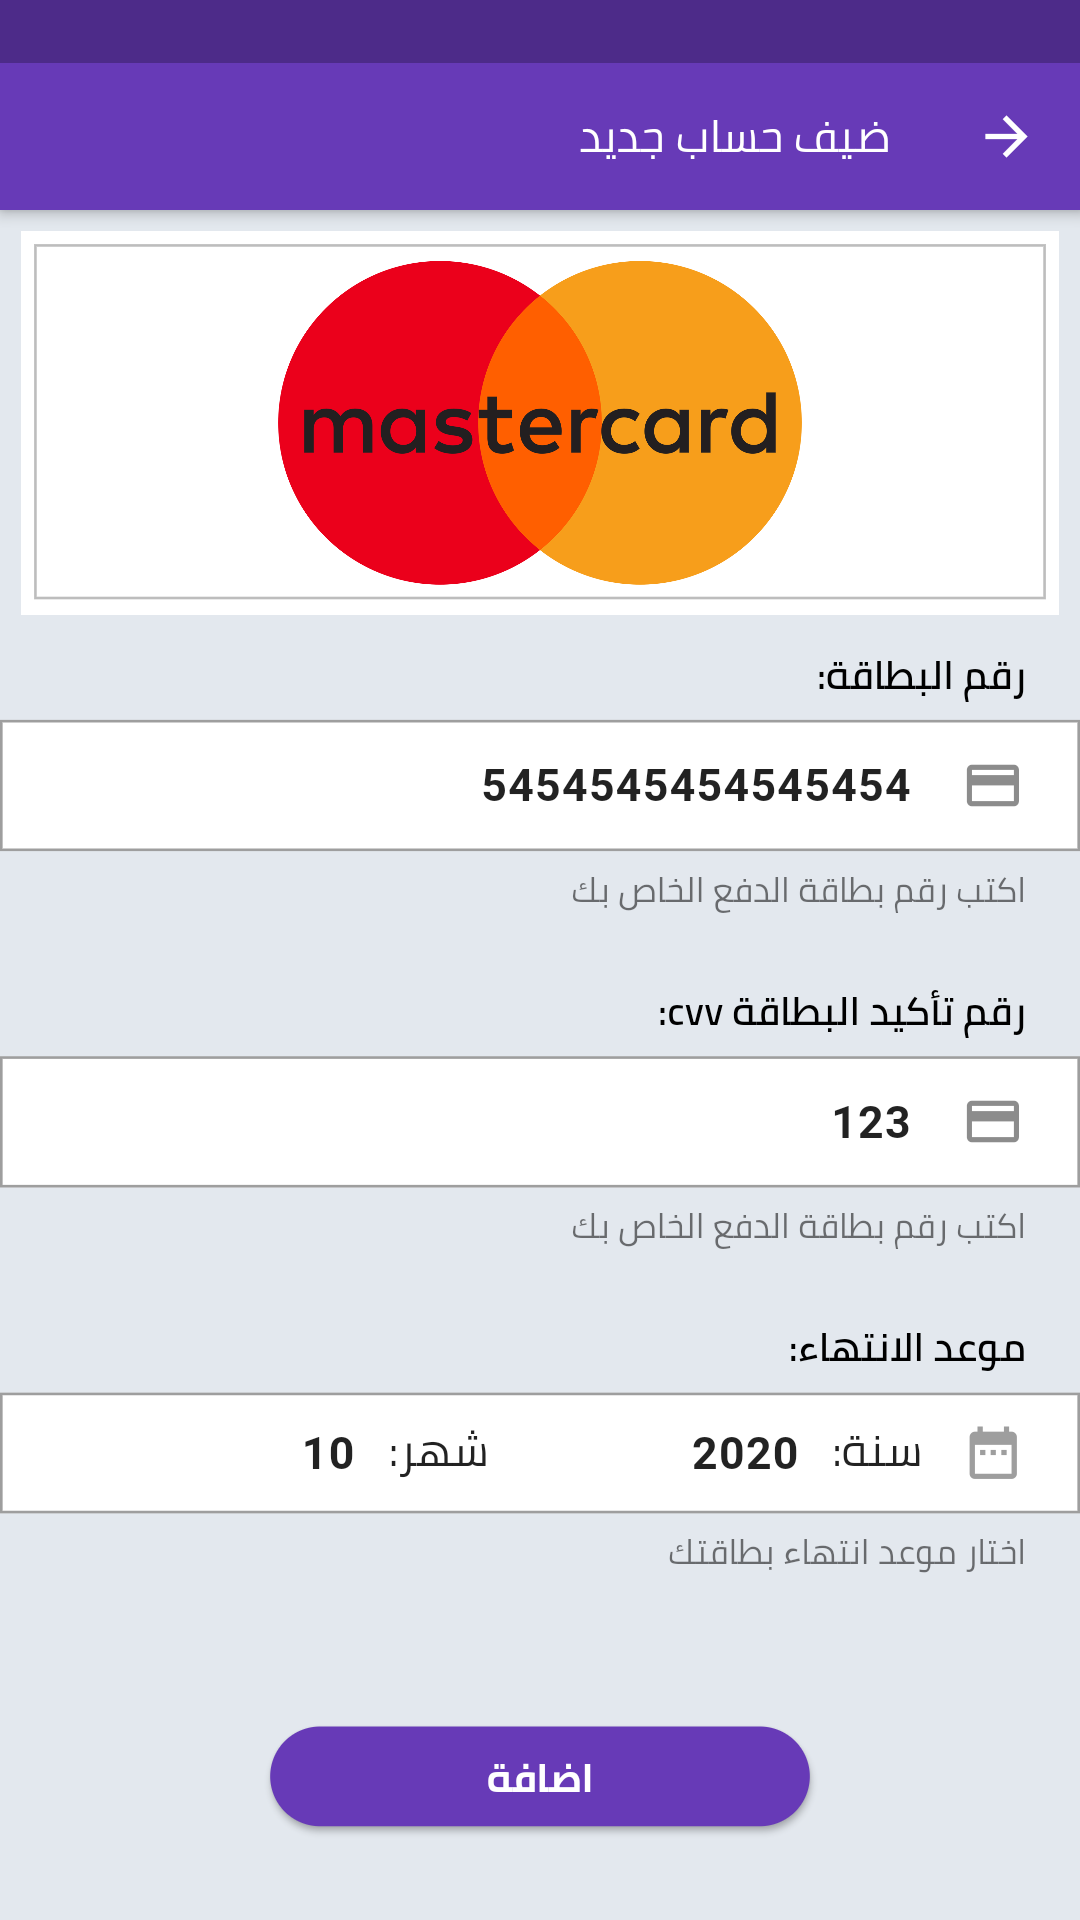
\includegraphics[width=0.5\linewidth]{images/ch3/payment/Adding Payment Method/5.png}
  
  \end{subfigure}%%
   \begin{subfigure}[b]{0.5\linewidth}
    \centering
    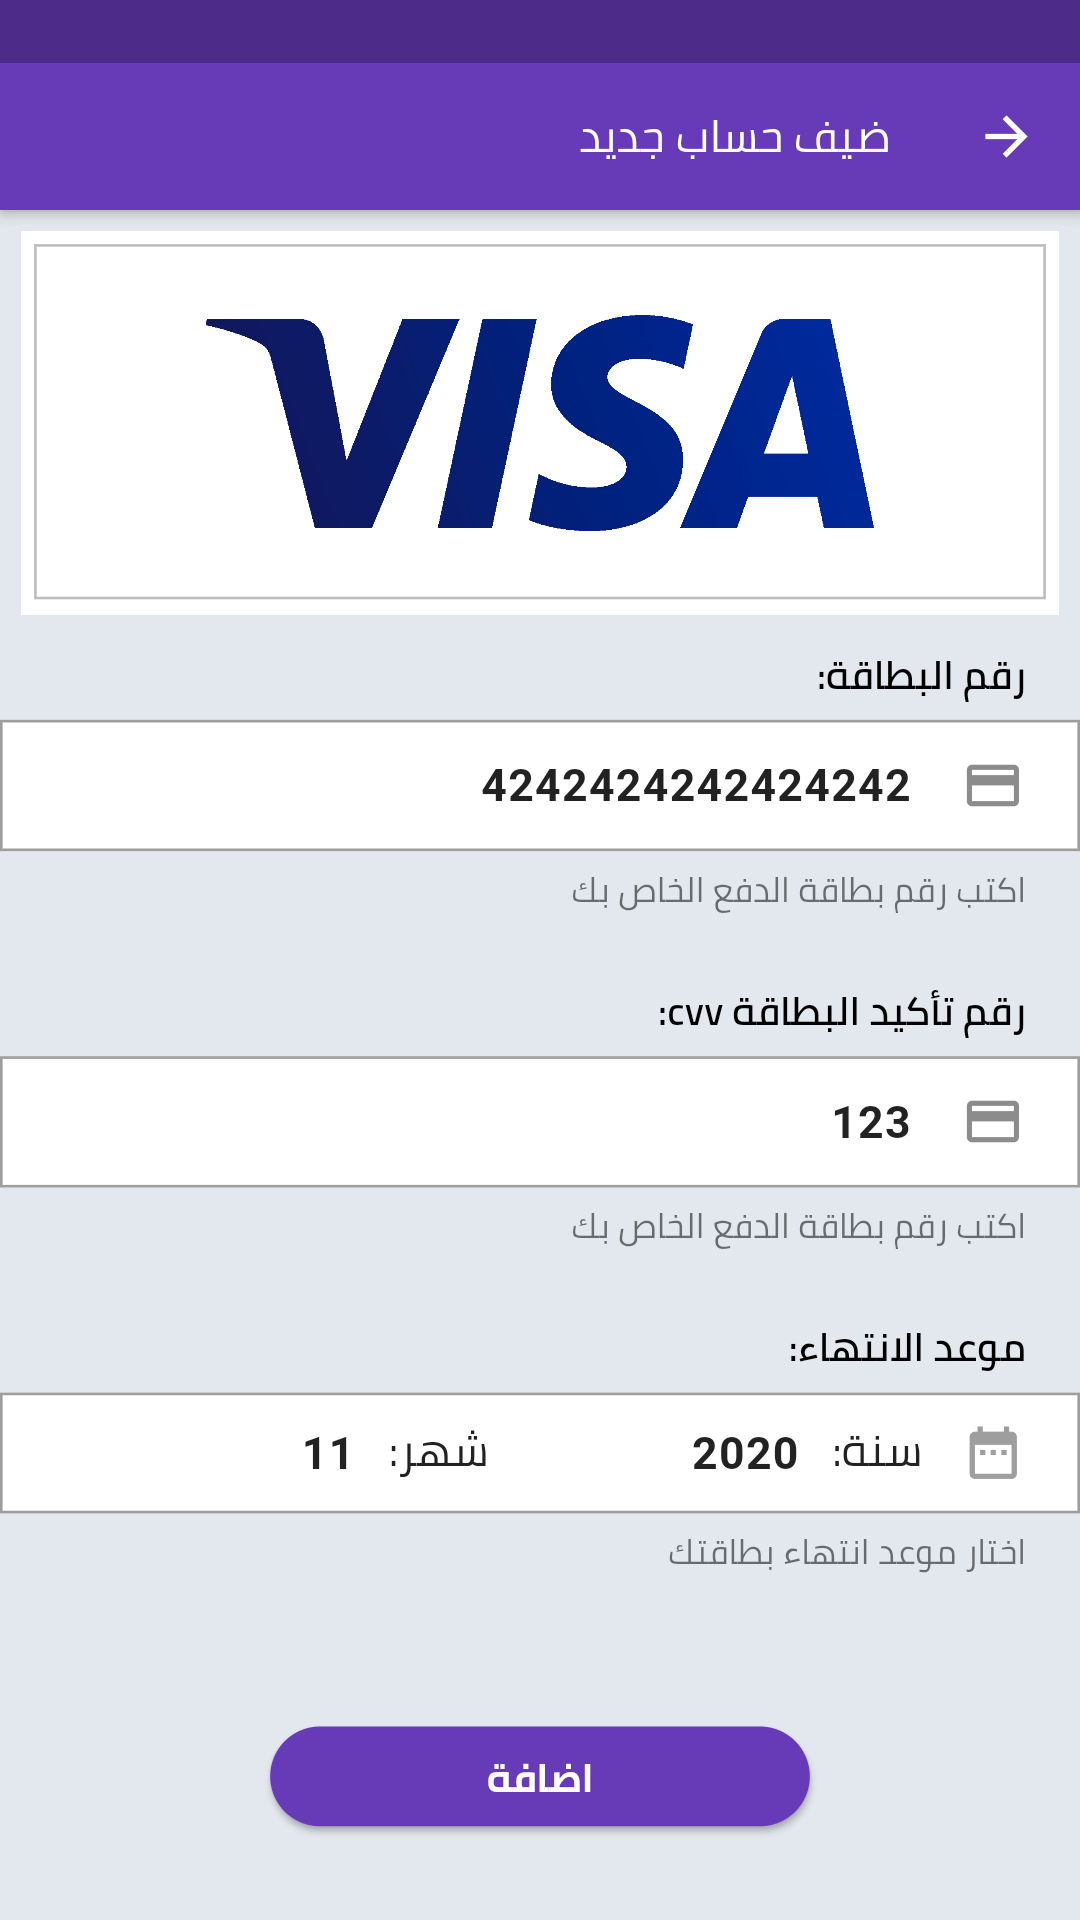
\includegraphics[width=0.5\linewidth]{images/ch3/payment/Adding Payment Method/2.png}
  
  \end{subfigure}%%
\caption{Payment Methods page}
  \end{figure}
